% ============================================================
% Beamer — ISLP Lecture Series — IMPROVED EDITION
% Advanced module A6: Survival Analysis and Censored Data (was ISLP Ch. 11)
% ============================================================
\documentclass[aspectratio=169,11pt]{beamer}
\usepackage[utf8]{inputenc}\usepackage[T1]{fontenc}\usepackage[english]{babel}
\usepackage{graphicx}\usepackage{booktabs}\usepackage{amsmath,amssymb,amsfonts}
\usepackage{mathtools}\usepackage{hyperref}\usepackage{xcolor}\usepackage{colortbl}
\usepackage{verbatim}\usepackage{alltt}
\usepackage{tikz}\usetikzlibrary{calc,arrows.meta,positioning,shapes}
\usepackage{tcolorbox}\tcbuselibrary{skins}

\usetheme{Madrid}\usecolortheme{default}
\setbeamertemplate{navigation symbols}{}
\setbeamertemplate{footline}[frame number]
\setbeamertemplate{blocks}[rounded][shadow=false]
\setbeamertemplate{headline}{%
  \leavevmode\hbox{%
    \begin{beamercolorbox}[wd=\paperwidth,ht=2.2ex,dp=0.9ex]{section in head/foot}%
      {\fontsize{4.6}{5.2}\selectfont%
       \insertsectionnavigationhorizontal{\paperwidth}{}{\hskip0pt plus1filll}}%
    \end{beamercolorbox}}%
}
\setbeamerfont{section in head/foot}{size=\tiny}
\setbeamerfont{palette primary}{size=\tiny}
\setbeamerfont{palette tertiary}{size=\tiny}
\setbeamerfont{section in toc}{size=\footnotesize}

\usepackage{listings}
\definecolor{pyKw}{RGB}{0,0,180}\definecolor{pyStr}{RGB}{20,120,40}
\definecolor{pyCom}{RGB}{120,120,120}\definecolor{accent}{RGB}{38,70,140}
\lstdefinestyle{Pystyle}{language=Python,basicstyle=\ttfamily\footnotesize,
  keywordstyle=\color{pyKw}\bfseries,commentstyle=\color{pyCom}\itshape,
  stringstyle=\color{pyStr},showstringspaces=false,upquote=true,
  columns=fullflexible,breaklines=true,literate={~}{{$\sim$}}1}
\lstset{style=Pystyle}

% Tighter TOC spacing (8 sections + appendix do not fit at default spacing)
\usepackage{etoolbox}
\makeatletter
\patchcmd{\beamer@sectionintoc}{\vskip1.5em}{\vskip.6em}{\typeout{TOCPATCH-OK}}{\typeout{TOCPATCH-FAIL}}
\makeatother

\AtBeginSection[]{\begin{frame}{Outline}\footnotesize
  \tableofcontents[currentsection,sectionstyle=show/shaded,subsectionstyle=show/show/hide]
\end{frame}}

\newcommand{\islpsource}[1]{%
  \vfill\hfill{\tiny\itshape\color{gray}Source: #1 \textemdash{} ISLP, James et al.\ (2023).}\par
}

\newtcolorbox{takeaway}[1][Takeaway]{enhanced,colback=green!4,colframe=green!50!black,
  boxrule=0pt,leftrule=2.5pt,arc=2pt,fonttitle=\bfseries,title=#1,
  left=2mm,right=2mm,top=1mm,bottom=1mm}
\newtcolorbox{numexample}[1][Worked example]{enhanced,colback=orange!4,colframe=orange!70!black,
  boxrule=0pt,leftrule=2.5pt,arc=2pt,fonttitle=\bfseries,title=#1,
  left=2mm,right=2mm,top=1mm,bottom=1mm}
\newtcolorbox{readme}[1][How to read this]{enhanced,colback=blue!4,colframe=accent,
  boxrule=0pt,leftrule=2.5pt,arc=2pt,fonttitle=\bfseries,title=#1,
  left=2mm,right=2mm,top=1mm,bottom=1mm}

\title{Quantitative Research Methods}
\subtitle{Survival Analysis and Censored Data\\[2pt]{\small Advanced module A6 --- optional self-study}}
\author{Prof.\ Dr.\ Christoph Weisser}
\date{}\graphicspath{{images/}}

\newtcolorbox{exercise}[1][Exercise]{enhanced, fontupper=\footnotesize, colback=purple!4, colframe=purple!55!black, boxrule=0pt, leftrule=2.5pt, arc=2pt, fonttitle=\bfseries, title=#1, left=2mm, right=2mm, top=1mm, bottom=1mm}
\newtcolorbox{solutionbox}[1][Solution]{enhanced, fontupper=\footnotesize, colback=teal!5, colframe=teal!55!black, boxrule=0pt, leftrule=2.5pt, arc=2pt, fonttitle=\bfseries, title=#1, left=2mm, right=2mm, top=1mm, bottom=1mm}
\newtcolorbox{longexercise}[1][Extended exercise (15 min)]{enhanced, fontupper=\footnotesize, colback=violet!6, colframe=violet!55!black, boxrule=0pt, leftrule=3pt, arc=2pt, fonttitle=\bfseries, title=#1, left=2mm, right=2mm, top=1mm, bottom=1mm}

% Reclaim ~2pt of body height (custom nav headline makes full slides tip over by ~1.83pt)
\addtobeamertemplate{frametitle}{}{\vspace{-2pt}}

\newtcolorbox{labnote}[1][Run this live in the lab notebook]{enhanced, fontupper=\footnotesize, colback=cyan!7, colframe=cyan!45!black, boxrule=0pt, leftrule=3pt, arc=2pt, fonttitle=\bfseries, title=#1, left=2mm, right=2mm, top=1mm, bottom=1mm}

% Industry application callout box --- slate grey, for real business/industry use
\definecolor{industryC}{RGB}{88,98,116}
\newtcolorbox{industry}[1][In industry]{enhanced, fontupper=\footnotesize, colback=industryC!7, colframe=industryC, boxrule=0pt, leftrule=3pt, arc=2pt, fonttitle=\bfseries, title={In industry --- #1}, left=2mm, right=2mm, top=1mm, bottom=1mm}

% Common-mistake callout --- crimson, for the error to pre-empt
\newtcolorbox{mistake}[1][Common mistake]{enhanced, fontupper=\footnotesize, colback=red!4, colframe=red!60!black, boxrule=0pt, leftrule=3pt, arc=2pt, fonttitle=\bfseries, title=#1, left=2mm, right=2mm, top=1mm, bottom=1mm}

\begin{document}
\begin{frame}[plain]\titlepage\end{frame}

\begin{frame}{The advanced modules at a glance}
  \vspace{-1.5mm}
  \begin{center}
  \scriptsize
  \setlength{\tabcolsep}{5pt}
  \renewcommand{\arraystretch}{1.30}
  \begin{tabular}{@{\hspace{2pt}}l >{\raggedright\arraybackslash}p{0.72\textwidth}@{\hspace{2pt}}}
    \toprule
    \textbf{Module} & \textbf{Topic} \\
    \midrule
     {\color{accent}A1} & Randomised Controlled Trials\,{\color{black!45}--- potential outcomes, randomisation, power} \\
    \rowcolor{black!3} {\color{accent}A2} & Explainable AI with Shapley Values\,{\color{black!45}--- axioms, exact and Monte-Carlo Shapley} \\
     {\color{accent}A3} & Conformal Prediction\,{\color{black!45}--- split conformal, CQR, prediction sets} \\
    \rowcolor{black!3} {\color{accent}A4} & GLMs and Splines\,{\color{black!45}--- exponential family, overdispersion, P-splines} \\
     {\color{accent}A5} & Support Vector Machines\,{\color{black!45}--- margins, the cost $C$, kernels} \\
    \rowcolor{accent!18} \textbf{A6} & \textbf{Survival Analysis}\,{\color{accent!75!black}--- censoring, Kaplan--Meier, Cox} \\
     {\color{accent}A7} & Multiple Testing\,{\color{black!45}--- FWER, Bonferroni and Holm, FDR} \\
    \bottomrule
  \end{tabular}
  \end{center}
  \vspace{2mm}
  {\scriptsize Seven optional, self-study modules that sit outside the taught
  chapter plan; today's module is highlighted. Each is a full deck in the course
  house style with a companion lab notebook.\par\medskip This module assumes Chapter 0 (distributions and tests), Chapter 3 (regression) and Chapter 4 (logistic regression). It was ISLP Chapter 11 in earlier editions of this course.}
\end{frame}


\begin{frame}{Contents}\small\tableofcontents[hideallsubsections]
  \vfill
  {\tiny Optional and advanced material is collected in the \textbf{appendix} at the end of the deck.}
\end{frame}

\begin{frame}{Notation in this chapter}
  \scriptsize
  \begin{center}
  \begin{tabular}{@{}ll@{}}
    \toprule
    \textbf{Symbol} & \textbf{Meaning} \\
    \midrule
    $T$ & the true event time --- what we want, but often do not see \\
    $C$ & the censoring time (end of study, drop-out, last contact) \\
    $Y=\min(T,C)$ & the \emph{observed} time for a subject \\
    $\delta=\mathbf{1}\{T\le C\}$ & event indicator: $1$ if the event was seen, $0$ if censored \\
    $S(t)=\Pr(T>t)$ & survival function: chance of surviving beyond $t$ \\
    $h(t)$ & hazard: instantaneous event rate at $t$ among those still at risk \\
    $H(t)=\int_0^t h(u)\,du$ & cumulative hazard, with $S(t)=e^{-H(t)}$ \\
    $t_1<\cdots<t_K$ & the distinct times at which events are observed \\
    $d_k$ & number of events at $t_k$ \\
    $r_k$ & number \emph{at risk} just before $t_k$ (alive and still followed) \\
    $\hat S(t)$ & the Kaplan--Meier (product-limit) estimator \\
    $O_1,E_1,V_1$ & observed, expected and variance of group-1 events (log-rank) \\
    $x_i,\ \beta$ & covariate vector of subject $i$; vector of log hazard ratios \\
    $h_0(t)$ & baseline hazard --- the part the Cox model never estimates \\
    $R(t)$ & risk set at $t$: $\{i : Y_i\ge t\}$ \\
    $\mathrm{PL}(\beta)$ & Cox partial likelihood \\
    $\mathrm{HR}=e^{\beta_j}$ & hazard ratio for a one-unit increase in $x_j$ \\
    \bottomrule
  \end{tabular}
  \end{center}
  {\tiny ISLP writes the distinct event times $d_1<\cdots<d_K$ with $q_k$ events and $r_k$ at risk; we use $t_k$, $d_k$, $r_k$ to keep $\delta$ free for the event indicator.}
\end{frame}

\begin{frame}{Sources and references}
  \begin{block}{Primary textbook}
    James, G., Witten, D., Hastie, T., Tibshirani, R., \& Taylor, J.\ (2023).
    \emph{An Introduction to Statistical Learning, with Applications in
    Python.} Springer.
  \end{block}
  \begin{readme}[Data used in this chapter]
    \textbf{BrainCancer} --- $88$ patients treated with stereotactic radiation, followed for up
    to $82.6$ months; $35$ deaths and $53$ censored observations. \textbf{Publication} ---
    time from completion to publication for $244$ clinical trials funded by the US NHLBI.
    Both ship with the course as CSV files.
  \end{readme}
\end{frame}

\begin{frame}{Learning objectives}
  By the end of this chapter you will be able to:
  \begin{itemize}
    \item \textbf{Explain} why censored outcomes break ordinary regression and
          classification, and what right-censoring means formally.
    \item \textbf{State} the independent-censoring assumption and recognise
          settings in which it fails.
    \item \textbf{Compute} a Kaplan--Meier curve by hand and read a median,
          a survival probability and a confidence band off it.
    \item \textbf{Apply} the log-rank test to compare two survival curves, and
          say what it cannot detect.
    \item \textbf{Fit and interpret} a Cox proportional-hazards model, reading
          $e^{\hat\beta_j}$ as a hazard ratio.
    \item \textbf{Check} the proportional-hazards assumption and \textbf{choose}
          a remedy when it fails.
  \end{itemize}
\end{frame}

\begin{frame}{Roadmap of this chapter}
  \begin{takeaway}[Learning from data you have only partly seen]
    \begin{enumerate}
      \item The problem: the response is a \emph{time}, and for many subjects the
            clock is still running.
      \item Censoring, stated properly --- and the one assumption everything rests on.
      \item The survival curve and its Kaplan--Meier estimate.
      \item Comparing two curves: the log-rank test.
      \item Adding covariates: the Cox proportional-hazards model.
      \item Practice: checking proportional hazards, and what to do when it fails.
    \end{enumerate}
  \end{takeaway}
\end{frame}

\begin{frame}{Where this chapter is used in industry}
  \scriptsize
  \begin{center}
  \begin{tabular}{@{}p{2.6cm}p{5.2cm}p{4.6cm}@{}}
    \toprule
    \textbf{Sector} & \textbf{Concrete application} & \textbf{Which decision it drives} \\
    \midrule
    Pharma, medtech & Overall and progression-free survival in oncology trials &
      Whether the drug goes to the regulator at all \\
    Subscription tech & Time to churn for customers who have \emph{not yet} churned &
      Retention spend, and which cohorts get it \\
    Banking, credit & Time to default or to early repayment on a loan book &
      Provisioning, pricing, and prepayment risk \\
    Insurance & Time to lapse of a policy; time to claim &
      Reserving and commission clawback rules \\
    Manufacturing & Time to failure of a component still in the field &
      Warranty terms and maintenance intervals \\
    HR analytics & Time to resignation among current employees &
      Which retention interventions are funded \\
    \bottomrule
  \end{tabular}
  \end{center}
  \begin{industry}[The common thread]
    In every row the interesting subjects are the ones \emph{nothing has happened to yet}.
    A churn model that quietly drops all still-active customers is trained on the unhappy
    minority; a warranty analysis that ignores components still running will promise a
    shorter life than the product has.
  \end{industry}
\end{frame}

\begin{frame}{Industry case in depth: a subscription business models churn}
  \footnotesize
  \begin{industry}[The data as it actually arrives]
    A SaaS firm has $180$ months of history. For a customer who cancelled in month $14$ the
    response is unambiguous: $T=14$. For a customer who signed up eight months ago and is
    still paying, all we know is $T>8$ --- a \textbf{right-censored} observation. At any
    snapshot the majority of the book is censored, and the newest, fastest-growing cohorts
    are censored the most heavily.
  \end{industry}
  \begin{readme}[Why the naive pipeline fails --- and what replaces it]
    The tempting shortcut is a classifier for ``churned in the last 12 months, yes/no''. It
    throws away \emph{when}, cannot use customers with less than $12$ months of tenure, and
    silently changes definition every time the snapshot moves. The survival framing keeps
    every customer: Kaplan--Meier for the cohort curve, Cox for the drivers, and the fitted
    curve integrates into an expected customer lifetime.
  \end{readme}
  \begin{takeaway}[Who signs off --- and the honest caveat]
    Finance owns the resulting lifetime-value number, so the curve has to be defensible.
    The caveat: customers who leave \emph{because} a price rise is coming are not censored
    independently of their risk --- and no amount of estimation fixes that.
  \end{takeaway}
\end{frame}

% ============================================================
\section{The Problem}
% ============================================================

\begin{frame}{The response is a time, and part of it is missing}
  We observe subjects from a starting point and wait for an \textbf{event}: death,
  churn, default, failure, publication.
  \begin{readme}[Three questions of exactly this shape]
    \begin{itemize}
      \item \emph{What fraction of these patients will still be alive in two years?}
      \item \emph{Do men and women in this cohort have the same survival?}
      \item \emph{Holding tumour type fixed, how much does a ten-point drop in the
            Karnofsky score raise the death rate?}
    \end{itemize}
  \end{readme}
  \begin{takeaway}
    The complication is not the response's \emph{type} --- times are just positive
    numbers --- but that for many subjects the event \textbf{has not happened yet}.
    Their true time $T$ is unknown; we only know it exceeds what we have watched.
  \end{takeaway}
\end{frame}

\begin{frame}{Why the tools we already have fail}
  \begin{center}\footnotesize
  \begin{tabular}{@{}p{3.5cm}p{4.1cm}p{4.7cm}@{}}
    \toprule
    \textbf{Naive framing} & \textbf{What it does with a subject still at risk} &
    \textbf{Why the answer is wrong} \\
    \midrule
    Linear regression of $Y$ on $x$ & treats the last-seen time as the event time &
    every censored $Y$ is \emph{too small}; the fit is biased downwards \\
    Classification ``event by $t^\star$?'' & needs a label it does not have for
    anyone followed less than $t^\star$ & discards recent subjects; the label
    changes whenever the snapshot moves \\
    Mean of the observed $Y_i$ & averages true times with truncated ones &
    estimates nothing in particular \\
    \bottomrule
  \end{tabular}
  \end{center}
  \begin{takeaway}
    Censoring is \textbf{not} missing data that we may drop or impute casually.
    Each censored subject carries real information --- ``survived at least this
    long'' --- and survival analysis is the machinery for spending it.
  \end{takeaway}
\end{frame}

\begin{frame}{BrainCancer: the data we will use all chapter}
  \footnotesize
  \begin{center}
  \begin{tabular}{@{}lll@{}}
    \toprule
    \textbf{Variable} & \textbf{Meaning} & \textbf{Values} \\
    \midrule
    \texttt{time}      & months of follow-up, $Y_i$ & $0.07$ to $82.56$ \\
    \texttt{status}    & event indicator $\delta_i$ & $1=$ died ($35$), $0=$ censored ($53$) \\
    \texttt{sex}       & patient sex & Female $45$, Male $43$ \\
    \texttt{diagnosis} & tumour type & Meningioma $42$, HG glioma $22$, Other $14$, LG glioma $9$ \\
    \texttt{ki}        & Karnofsky performance index & $40$--$100$; higher is healthier \\
    \texttt{gtv}       & gross tumour volume, cm$^3$ & $0.01$--$34.64$ \\
    \texttt{loc}       & tumour location & Supratentorial $69$, Infratentorial $19$ \\
    \texttt{stereo}    & radiation method & SRT $65$, SRS $23$ \\
    \bottomrule
  \end{tabular}
  \end{center}
  \begin{mistake}[Establish the coding before anything else]
    We checked the coding against the data, not against memory: with $\delta=1$ read as
    \emph{death} the sex log-rank statistic is $1.44$, exactly ISLP's published value.
    Read the other way round every curve in the chapter inverts silently. $60.2\%$ of
    these patients are censored --- one missing \texttt{diagnosis} leaves $87$ complete
    cases for the Cox fit.
  \end{mistake}
\end{frame}

\begin{frame}{Three tempting shortcuts, and the damage each does}
  \footnotesize
  \begin{numexample}[Median survival on BrainCancer --- four ways]
    \begin{itemize}
      \item[(a)] \textbf{Drop the $53$ censored patients.} The $35$ remaining deaths have
            median $11.6$ months. But dropping the censored keeps only patients who died
            \emph{during} the study --- the short-lived ones --- so survival is far
            \textbf{understated}.
      \item[(b)] \textbf{Call the censoring time a death.} All $88$ ``events'' give median
            $23.7$ months. Every censored $Y_i$ is a lower bound treated as exact, so this
            still \textbf{understates} survival.
      \item[(c)] \textbf{Assume the censored never die.} Then $\hat S(24)=1-25/88=0.716$
            and the curve flattens at $1-35/88=0.602$: the median is \emph{never reached}.
            Survival is \textbf{overstated}.
      \item[$\Rightarrow$] \textbf{Kaplan--Meier} uses all $88$ patients honestly:
            median $\mathbf{47.8}$ months, with $\hat S(24)=0.683$.
    \end{itemize}
  \end{numexample}
  \begin{takeaway}
    Two of the shortcuts halve the answer and one inflates it. The errors do not
    cancel, and none of them get smaller with more data.
  \end{takeaway}
\end{frame}

\begin{frame}{The same four estimates, drawn}
  \footnotesize
  \begin{center}
    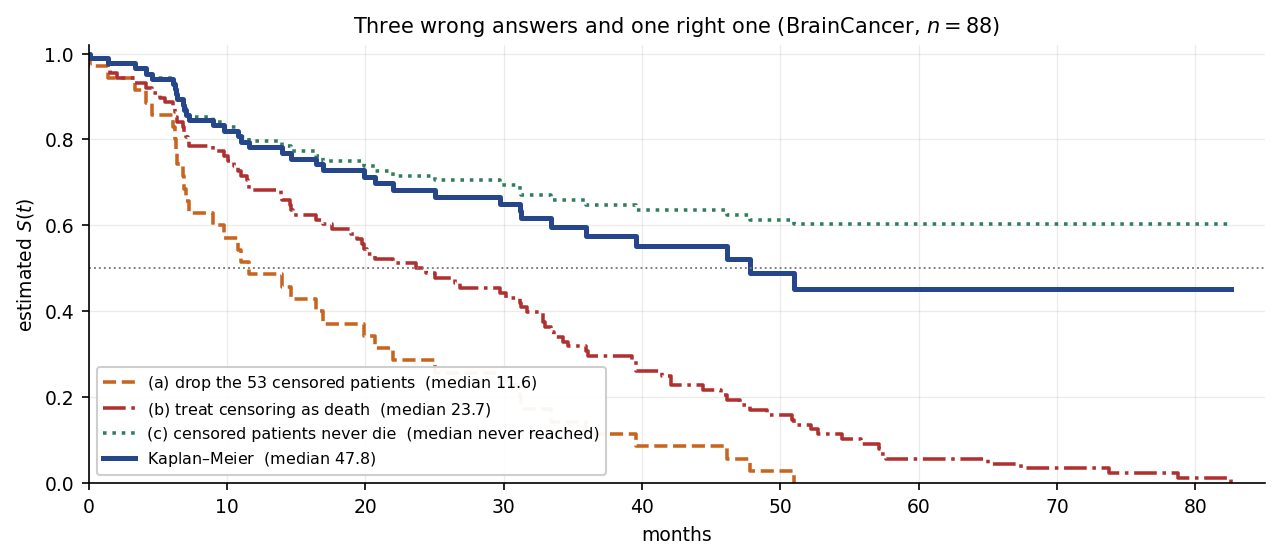
\includegraphics[width=0.92\textwidth,height=0.53\textheight,keepaspectratio]{ch11_naive.png}
  \end{center}
  \begin{takeaway}
    The Kaplan--Meier curve (thick blue) crosses $0.5$ at $47.8$ months. Shortcut (a)
    crosses at $11.6$ and (b) at $23.7$; shortcut (c) never gets below $0.602$. Same
    $88$ patients, four different stories.
  \end{takeaway}
\end{frame}

% ------------------------------------------------------------
\begin{frame}{Exercise 11.1 --- Why the shortcuts fail [Concept]}
\begin{exercise}
  A streaming service has $10\,000$ subscribers. In the last year $1\,200$ cancelled;
  the rest are still subscribed, with tenures ranging from one week to nine years.
  An analyst wants ``the average subscription length''.
  \begin{enumerate}
    \item The analyst averages the tenure of the $1\,200$ who cancelled. In which
          direction is the answer biased, and why?
    \item A colleague instead averages current tenure over all $10\,000$. In which
          direction is \emph{that} biased?
    \item Which single piece of information does every still-subscribed customer
          contribute, and why is it not nothing?
    \item Give one reason why a classifier for ``cancelled within 12 months?'' is a
          poor substitute.
  \end{enumerate}
\end{exercise}
\end{frame}

\begin{frame}{Solution --- Exercise 11.1}
\begin{solutionbox}
  \textbf{Method.} Ask, for each proposal, \emph{which subjects it keeps} and whether that
  selection is related to the outcome. Selection on the outcome is what creates the bias.

  \medskip
  \textbf{Part 1 --- cancellers only: biased downwards.} To have cancelled inside a
  one-year window you must have had a short subscription. Long-lived customers are
  systematically excluded, so the average is far too small --- exactly shortcut (a),
  which gave $11.6$ instead of $47.8$ months on BrainCancer.

  \medskip
  \textbf{Part 2 --- current tenure for everyone: also biased downwards.} For an active
  customer, current tenure is a \emph{lower bound} on the eventual subscription length.
  Averaging lower bounds as if they were the truth understates the mean --- shortcut (b).

  \medskip
  \textbf{Part 3 --- what a censored subject tells us.} That $T_i>Y_i$. Concretely, an
  active customer of $30$ months' tenure proves at least one customer survives past
  $30$ months, and belongs in the \emph{risk set} at every time up to $30$. Kaplan--Meier
  and Cox both use exactly this.

  \medskip
  \textbf{Part 4 --- against the classifier.} Anyone who joined less than $12$ months ago
  has no label at all, so the newest cohorts are silently dropped; and the target changes
  meaning every time the snapshot date moves.
\end{solutionbox}
\end{frame}

% ============================================================
\section{Censoring}
% ============================================================

\begin{frame}{The censoring picture --- the figure to keep in your head}
  \footnotesize
  \begin{center}
    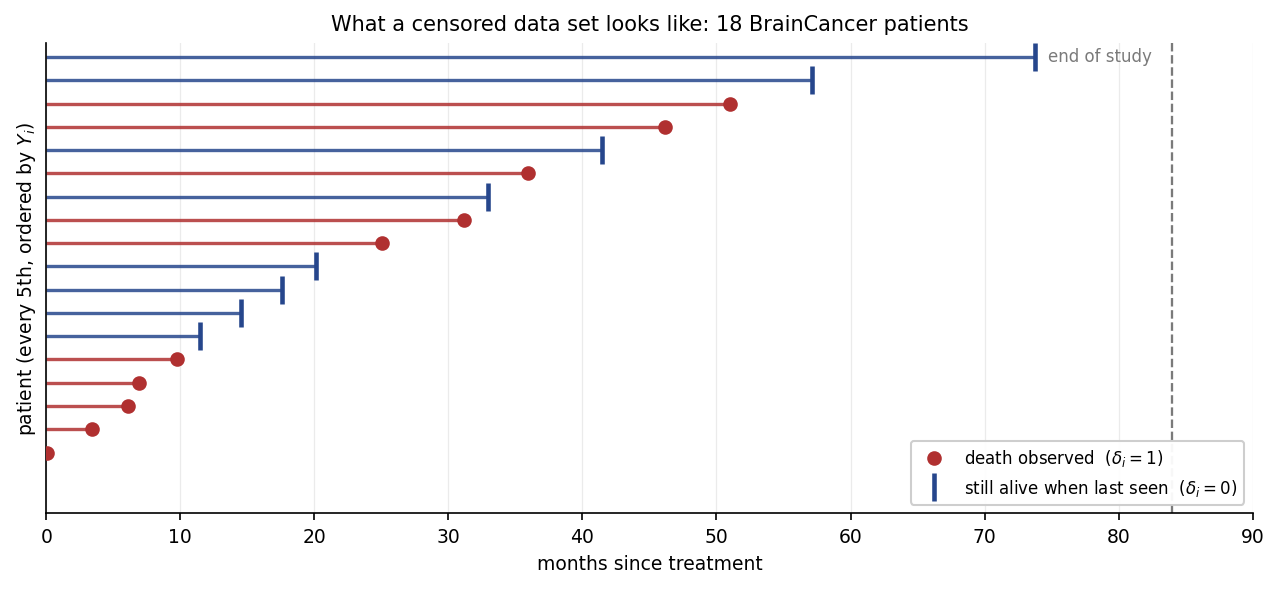
\includegraphics[width=0.94\textwidth,height=0.53\textheight,keepaspectratio]{ch11_censoring.png}
  \end{center}
  \begin{takeaway}
    Each bar is one patient's follow-up. A \textbf{dot} ends a bar where a death was seen
    ($\delta_i=1$): the time is exact. A \textbf{tick} ends a bar where the patient was
    last seen alive ($\delta_i=0$): the true $T_i$ lies somewhere to the \emph{right} of
    the tick, and we will never know where.
  \end{takeaway}
\end{frame}

\begin{frame}{What we actually observe}
  \footnotesize
  \begin{block}{The observed pair}
    \[
      \boxed{\;Y_i=\min(T_i,\,C_i),\qquad
              \delta_i=\mathbf{1}\{T_i\le C_i\}.\;}
    \]
  \end{block}
  \begin{readme}
    \begin{itemize}
      \item $T_i$ is the \textbf{event time} we care about; $C_i$ is the
            \textbf{censoring time} at which observation stops for reasons other than
            the event.
      \item We never see both. We see whichever comes first, $Y_i$, plus a flag
            $\delta_i$ saying which one it was.
      \item $\delta_i=1$: the event happened at $Y_i$, so $T_i=Y_i$ exactly.
      \item $\delta_i=0$: \textbf{right-censored} --- all we learn is $T_i>Y_i$.
      \item A data set is therefore a list of pairs $(Y_i,\delta_i)$, plus covariates.
    \end{itemize}
  \end{readme}
  \begin{takeaway}
    Every method in this chapter is a way of reading the likelihood of the pair
    $(Y_i,\delta_i)$ rather than of $T_i$.
  \end{takeaway}
\end{frame}

\begin{frame}{The one assumption the whole chapter rests on}
  \scriptsize
  \begin{block}{Independent (non-informative) censoring}
    \[
      \boxed{\;T_i \perp C_i \;\big|\; x_i \;}
    \]
    Given the covariates, \emph{when} a subject stops being observed carries no
    information about \emph{when} their event would have occurred.
  \end{block}
  \begin{readme}
    \begin{itemize}
      \item Equivalently: a subject censored at time $t$ is representative of everyone
            still at risk at $t$. That is what lets us drop them from the risk set and
            carry on.
      \item It holds by construction for \textbf{administrative censoring} --- the study
            ended, the extract was pulled --- because the calendar does not know who is ill.
      \item It is an \textbf{assumption}, not a property of the data. No amount of data
            tests it: the counterfactual $T_i$ for a censored subject is never observed.
    \end{itemize}
  \end{readme}
  \begin{takeaway}
    Without it, none of Kaplan--Meier, log-rank or Cox estimates what we think it does.
    State it explicitly; then argue for it from how the data were collected.
  \end{takeaway}
\end{frame}

\begin{frame}{When independent censoring fails}
  \footnotesize
  \begin{mistake}[The failure to watch for]
  \scriptsize
    Patients drop out of a trial \emph{because they are getting sicker} --- too unwell to
    travel to the clinic. Their censoring times cluster just before the deaths that would
    have followed. Removing them from the risk set removes the highest-risk subjects, so
    every subsequent conditional survival is too high and $\hat S(t)$ is
    \textbf{optimistic}.
  \end{mistake}
  \begin{readme}[Three more from ordinary business data]
    \begin{itemize}
      \item \textbf{Churn:} a customer whose card silently expires is recorded as active
            until the next billing cycle --- censoring caused by disengagement.
      \item \textbf{Credit:} a borrower who refinances elsewhere is censored, and
            refinancing is chosen by the borrowers least likely to default.
      \item \textbf{Warranty:} a component returned by a customer who has stopped using
            the product is censored precisely because it was never stressed.
    \end{itemize}
  \end{readme}
  \begin{takeaway}
    Ask of every censored record: \emph{why did observation stop?} ``The study ended''
    is safe. ``The subject withdrew'' needs a sensitivity analysis, and an honest
    sentence in the write-up.
  \end{takeaway}
\end{frame}

% ------------------------------------------------------------
\begin{frame}{Exercise 11.2 --- Reading $(Y,\delta)$ off a study [Math]}
\begin{exercise}
  A study opens on 1 January 2020 and closes on 31 December 2022 (all times in
  \emph{months from enrolment}). Four subjects:
  \begin{center}\footnotesize
  \begin{tabular}{@{}clll@{}}
    \toprule
    & \textbf{Enrolled} & \textbf{What happened} & \\
    \midrule
    A & month $0$  & event at month $18$ & \\
    B & month $0$  & alive and in the study at closure & \\
    C & month $12$ & moved abroad at month $9$ after enrolment & \\
    D & month $24$ & event at month $4$ after enrolment & \\
    \bottomrule
  \end{tabular}
  \end{center}
  \begin{enumerate}
    \item Give $(Y_i,\delta_i)$ for each subject.
    \item Which censoring here is administrative, and which is not?
    \item At time $t=10$ months, which subjects are in the risk set $R(10)$?
    \item Why is $\sum_i Y_i/4$ not an estimate of $E[T]$?
  \end{enumerate}
\end{exercise}
\end{frame}

\begin{frame}{Solution --- Exercise 11.2}
  \footnotesize
\begin{solutionbox}
  \scriptsize
  \textbf{Part 1 --- the observed pairs.} The study is open for $36$ months, so a subject
  enrolled in month $s$ can be followed for at most $36-s$ months.
  \[
    \begin{array}{c|c|c|c|l}
      \text{Subject} & C_i & Y_i=\min(T_i,C_i) & \delta_i & \text{reason}\\ \hline
      A & 36 & 18 & 1 & \text{event seen at }18 \\
      B & 36 & 36 & 0 & \text{still event-free at closure}\\
      C & 9  & 9  & 0 & \text{lost to follow-up at }9\\
      D & 12 & 4  & 1 & \text{event seen at }4
    \end{array}
  \]
  \textbf{Part 2 --- kind of censoring.} B is \textbf{administrative}: the calendar ran
  out, which cannot depend on B's risk. C is \textbf{loss to follow-up}; independence is
  now an argument, not a fact --- moving abroad is plausibly unrelated to the event, but
  it must be said out loud.

  \medskip
  \textbf{Part 3 --- the risk set at $t=10$.} $R(10)=\{i: Y_i\ge 10\}=\{A,B\}$. Subject C
  left at $9$ and D's event occurred at $4$; both are gone. Note D contributes to $R(4)$
  even though enrolled last --- the clock is time \emph{since enrolment}, not calendar time.

  \medskip
  \textbf{Part 4 --- why the naive mean fails.} $\tfrac14(18+36+9+4)=16.75$ mixes two exact
  times with two lower bounds. It is an average of $\min(T_i,C_i)$, which depends on the
  study design; enrol B a year earlier and the ``estimate'' changes although nothing about
  the disease did.
\end{solutionbox}
\end{frame}

% ============================================================
\section{Kaplan--Meier}
% ============================================================

\begin{frame}{The object of interest: the survival curve}
  \scriptsize
  \begin{block}{Definition}
    \[
      \boxed{\;S(t)=\Pr(T>t)\;}
      \qquad\text{a non-increasing function with } S(0)=1 .
    \]
  \end{block}
  \begin{readme}
    \begin{itemize}
      \item $S(t)$ answers the question a decision-maker actually asks: \emph{what
            fraction is still event-free at $t$?} And $1-S(t)$ is the cumulative
            incidence --- the chance the event has happened by $t$.
      \item The \textbf{median survival} is the smallest $t$ with $S(t)\le 0.5$.
      \item $S$ is a \emph{whole function}: two groups can share a median and differ
            everywhere else, so we plot curves before testing anything.
      \item The \textbf{mean} $E[T]=\int_0^\infty S(t)dt$ needs the entire tail: on
            BrainCancer $\hat S$ stops at $0.452$ after $82.56$ months, so anything beyond
            is extrapolation. Use the \textbf{restricted} mean
            $\mathrm{RMST}(\tau)=\int_0^\tau \hat S(t)dt$ instead --- $33.98$ months for
            $\tau=48$, $39.51$ for $\tau=60$.
    \end{itemize}
  \end{readme}
  \begin{takeaway}
    Quote a median, a probability at a stated horizon, or an RMST \emph{with} its horizon.
    A bare mean survival time from censored data is an extrapolation in disguise.
  \end{takeaway}
\end{frame}

\begin{frame}{The idea: chain the conditional survivals}
  \scriptsize
  Surviving past $t$ means surviving each earlier event time \emph{in turn}:
  \begin{block}{Decomposition}
    \[
      S(t_k)=\Pr(T>t_k)
            =\prod_{j=1}^{k}\underbrace{\Pr(T>t_j \mid T>t_{j-1})}_{\text{survive step }j}
    \]
  \end{block}
  \begin{readme}[Why this is the whole trick]
    \begin{itemize}
      \item Each factor is a \emph{conditional} probability, estimable from the subjects
            who reached $t_{j-1}$ --- and censored subjects reached it too.
      \item So a subject censored at $30$ months contributes to every factor up to
            month $30$ and simply leaves the risk set afterwards.
      \item Estimate factor $j$ by the obvious proportion: of the $r_j$ at risk,
            $d_j$ died, so $1-d_j/r_j$ survived.
    \end{itemize}
  \end{readme}
  \begin{takeaway}
    Censoring is handled by \textbf{shrinking the denominator}, not by deleting rows.
    That single move is what makes the estimator honest.
  \end{takeaway}
\end{frame}

\begin{frame}{The Kaplan--Meier (product-limit) estimator}
  \scriptsize
  \begin{block}{Rule}
    \[
      \boxed{\;\hat S(t)=\prod_{k\,:\,t_k\le t}\left(1-\frac{d_k}{r_k}\right)\;}
    \]
  \end{block}
  \begin{readme}
    \begin{itemize}
      \item $t_1<\cdots<t_K$ are the distinct times at which \textbf{events} occur ---
            censoring times never enter the product.
      \item $d_k$ = events at $t_k$; \ $r_k=\#\{i: Y_i\ge t_k\}$ = subjects at risk just
            before $t_k$.
      \item $\hat S$ is a \textbf{step function}: flat between event times, dropping by
            the factor $1-d_k/r_k$ at each $t_k$.
      \item Every censoring at time $c$ removes one subject from all later $r_k$, so the
            \emph{next} drop is bigger. That is how censored subjects influence the curve.
      \item With no censoring, $r_k$ falls by exactly $d_k$ each step and $\hat S$
            collapses to the empirical survival function $\#\{Y_i>t\}/n$.
    \end{itemize}
  \end{readme}
  \begin{takeaway}
    Non-parametric: no distribution for $T$, no model for the hazard, only the
    sequence of at-risk sets.
  \end{takeaway}
\end{frame}

\begin{frame}{By hand: the first three deaths in BrainCancer}
  \begin{numexample}[Three steps of the product]
    Ordered follow-up begins
    $0.07,\;1.18^{+},\;1.41,\;1.54^{+},\;2.03^{+},\;3.38,\dots$ ($^{+}$ marks censoring).
    \[
      \begin{array}{c|c|c|c|l}
        k & t_k & r_k & d_k & \hat S(t_k)\\ \hline
        1 & 0.07 & 88 & 1 & 1\cdot\tfrac{87}{88}=0.9886\\
        2 & 1.41 & 86 & 1 & 0.9886\cdot\tfrac{85}{86}=0.9771\\
        3 & 3.38 & 83 & 1 & 0.9771\cdot\tfrac{82}{83}=0.9654
      \end{array}
    \]
    Note $r_2=86$, not $87$: the censoring at $1.18$ removed a subject before $t_2$.
    Between $t_2$ and $t_3$ two more censorings ($1.54$, $2.03$) take $r$ from $85$ to $83$
    without the curve moving at all.
  \end{numexample}
  \begin{takeaway}
    Censorings are invisible in the \emph{numerator} and decisive in the
    \textbf{denominator}. Track $r_k$ carefully and the rest is arithmetic.
  \end{takeaway}
\end{frame}

\begin{frame}{The Kaplan--Meier curve with its confidence band}
  \footnotesize
  \begin{center}
    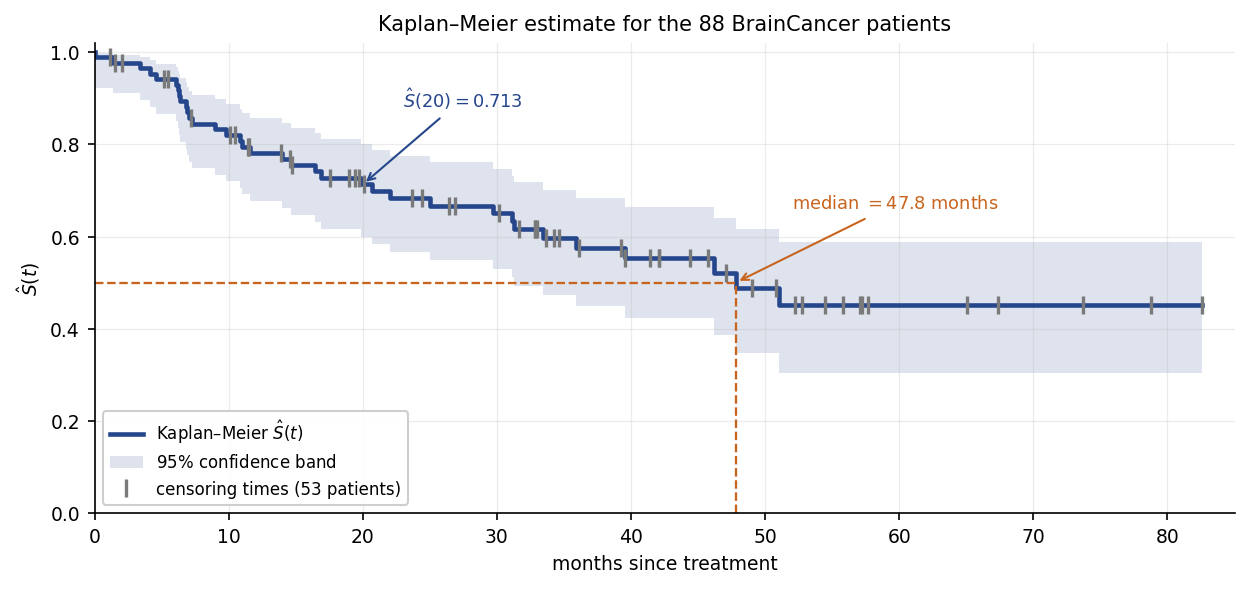
\includegraphics[width=0.9\textwidth,height=0.51\textheight,keepaspectratio]{ch11_km.png}
  \end{center}
  \begin{takeaway}
    Read off: $\hat S(20)=0.713$ with $95\%$ interval $[0.600,\,0.800]$, and a median of
    $47.8$ months. The band widens from left to right --- only $48$ of the $88$ patients
    are still under observation after month $20$ --- and the curve flattens at $0.452$
    because the last observation is censored, so it never reaches zero.
  \end{takeaway}
\end{frame}

\begin{frame}{Reading the curve without over-reading it}
  \begin{center}\footnotesize
  \begin{tabular}{@{}rcccc@{}}
    \toprule
    $t$ (months) & $10$ & $20$ & $40$ & $60$ \\
    \midrule
    $\hat S(t)$ & $0.821$ & $0.713$ & $0.552$ & $0.452$ \\
    $95\%$ interval & $[0.720,0.888]$ & $[0.600,0.800]$ & $[0.423,0.664]$ & $[0.305,0.587]$ \\
    \bottomrule
  \end{tabular}
  \end{center}
  \begin{readme}[Three habits]
    \begin{itemize}
      \item Quote $\hat S(t)$ \emph{with} its interval; the right-hand end of a survival
            curve is always thin data.
      \item The median comes with a one-sided story here: its $95\%$ interval is
            $[31.25,\ \infty)$, because $\hat S$ never gets far enough below $0.5$ to
            pin down an upper limit.
      \item Never extrapolate past the largest observed time ($82.56$ months).
    \end{itemize}
  \end{readme}
  \begin{industry}[Insurance: the flat tail is a modelling decision]
    A lapse curve that flattens at $0.45$ does not mean $45\%$ of policies last forever ---
    it means follow-up ran out. Reserving teams must either extrapolate with a parametric
    tail and say so, or report a restricted quantity such as $\mathrm{RMST}(\tau)$.
  \end{industry}
\end{frame}

\begin{frame}{Censored observations do not step the curve down}
  \footnotesize
  \begin{mistake}
  \scriptsize
    Reading each tick mark as a small drop. A censoring at time $c$ leaves $\hat S$
    \textbf{unchanged} --- nobody died. It only shrinks $r_k$ for all $t_k>c$, so the
    \emph{next} death causes a larger step. Many ticks in a row and then a big drop is
    the signature of thin data, not of a sudden hazard.
  \end{mistake}
  \begin{readme}[Two more honest readings]
    \begin{itemize}
      \item $\hat S$ reaches $0$ only if the \emph{largest} observation is an event. Here
            it is censored, so the curve stops at $0.452$ and the mean is not identified.
      \item If a group's curve never crosses $0.5$, its median survival is
            ``not reached'' --- report that, rather than the last value on the curve.
    \end{itemize}
  \end{readme}
  \begin{takeaway}
    Always plot the censoring marks. A curve without them hides how much of its
    right-hand side rests on a handful of patients.
  \end{takeaway}
\end{frame}

% ------------------------------------------------------------
\begin{frame}{Exercise 11.3 --- Kaplan--Meier by hand [Math]}
\begin{exercise}
  Six patients are followed (months, $^{+}$ = censored):
  \[
    4,\quad 6^{+},\quad 8,\quad 11^{+},\quad 12,\quad 15 .
  \]
  \begin{enumerate}
    \item Tabulate $t_k$, $r_k$, $d_k$ for every \emph{event} time.
    \item Compute $\hat S(t)$ at each event time.
    \item Give $\hat S(10)$ and the estimated median survival.
    \item Redo part 2 pretending the two censored patients had died at $6$ and $11$.
          Compare.
  \end{enumerate}
\end{exercise}
\end{frame}

\begin{frame}{Solution --- Exercise 11.3}
  \footnotesize
\begin{solutionbox}
  \scriptsize
  \textbf{Parts 1--2 --- the product.} Event times are $4,8,12,15$; $r_k$ counts everyone
  with $Y_i\ge t_k$.
  \[
    \begin{array}{c|c|c|c|l}
      k & t_k & r_k & d_k & \hat S(t_k)\\ \hline
      1 & 4  & 6 & 1 & 1\cdot(1-\tfrac16)=0.8333\\
      2 & 8  & 4 & 1 & 0.8333\cdot(1-\tfrac14)=0.6250\\
      3 & 12 & 2 & 1 & 0.6250\cdot(1-\tfrac12)=0.3125\\
      4 & 15 & 1 & 1 & 0.3125\cdot(1-\tfrac11)=0
    \end{array}
  \]
  At $t_2=8$ the risk set is $\{8,11^{+},12,15\}$, so $r_2=4$: the patient censored at
  $6$ has left, but was counted at $t_1$.

  \medskip
  \textbf{Part 3.} $\hat S$ is flat between event times, so $\hat S(10)=\hat S(8)=0.6250$.
  The median is the first $t$ with $\hat S(t)\le 0.5$, namely $t=\mathbf{12}$.

  \medskip
  \textbf{Part 4 --- censoring treated as death.} Now all six are events with
  $r=6,5,4,3,2,1$, giving $\hat S=\tfrac56,\tfrac46,\dots$, i.e.\ the plain empirical
  curve $5/6,\,4/6,\,3/6,\,2/6,\,1/6,\,0$ at $4,6,8,11,12,15$. The median falls to
  $\mathbf{11}$ and $\hat S(10)=4/6=0.667$ --- the curve is dragged down early and the
  median is understated, exactly shortcut (b) from the motivation.
\end{solutionbox}
\end{frame}

% ------------------------------------------------------------
\begin{frame}{Extended Exercise 11.1 --- Kaplan--Meier in Python [Python]}
\begin{longexercise}
  Using \texttt{BrainCancer} and \texttt{lifelines}:
  \begin{enumerate}
    \item Fit the overall Kaplan--Meier curve. Report $\hat S(20)$ with its $95\%$
          interval and the median survival time.
    \item Fit separate curves for men and women. Report each group's size, number of
          deaths and median.
    \item Plot both curves with censoring marks, and say in one sentence what the plot
          suggests.
    \item Verify by direct arithmetic that the first three steps of the overall curve
          are $0.9886$, $0.9771$, $0.9654$.
  \end{enumerate}
\end{longexercise}
\begin{labnote}[Run this live]
  The worked solution sits in \texttt{chapter\_11\_lab.ipynb} under
  \emph{Lecture exercises --- worked Python solutions}: the cell headed
  \emph{Extended Exercise 11.1 --- Kaplan--Meier in Python [Python]}.
\end{labnote}
\end{frame}

\begin{frame}[fragile]{Solution --- Extended Exercise 11.1 (1/2)}
\begin{solutionbox}[Solution --- code]
\begin{lstlisting}[basicstyle=\ttfamily\scriptsize]
import pandas as pd, numpy as np                     # data and arithmetic
from lifelines import KaplanMeierFitter              # product-limit estimator

BC = load('BrainCancer', index_col=0)                # 88 x 8; status 1 = death
km = KaplanMeierFitter().fit(BC['time'], BC['status'])   # censoring handled here
print('S(20) = %.4f' % km.survival_function_at_times(20).iloc[0])
print('95%% CI  ', np.round(km.confidence_interval_.loc[:20].iloc[-1].values, 4))
print('median  ', km.median_survival_time_)          # first t with S(t) <= 0.5

for s in ['Female', 'Male']:                         # one curve per group
    m = BC['sex'] == s
    k = KaplanMeierFitter().fit(BC.loc[m, 'time'], BC.loc[m, 'status'])
    print(s, 'n=%d deaths=%d median=%.2f'
          % (m.sum(), BC.loc[m, 'status'].sum(), k.median_survival_time_))

et = km.event_table                                  # r_k and d_k, tabulated
print(et.head(7)[['at_risk', 'observed', 'censored']])   # check the hand arithmetic
\end{lstlisting}
\end{solutionbox}
\end{frame}

\begin{frame}{Solution --- Extended Exercise 11.1 (2/2)}
  \footnotesize
\begin{solutionbox}[Solution --- output and reading]
  \scriptsize
  \textbf{Printout.}
  \begin{center}\ttfamily\footnotesize
  S(20) = 0.7132\quad 95\% CI [0.5996, 0.7998]\quad median 47.8\\[2pt]
  Female n=45 deaths=15 median=51.02\qquad Male n=43 deaths=20 median=31.25
  \end{center}
  \begin{itemize}
    \item \textbf{Part 1.} $71.3\%$ of patients are still alive at $20$ months; the
          interval $[0.600,0.800]$ is already $20$ percentage points wide with $88$
          patients --- survival curves are data-hungry.
    \item \textbf{Part 2--3.} The male median is $31.25$ months against $51.02$ for
          women, and the male curve sits below the female curve almost everywhere. The
          plot \emph{suggests} worse male survival; whether the gap is more than noise is
          the next section's question, and $45$ vs $43$ patients with $35$ deaths in total
          is not much evidence.
    \item \textbf{Part 4.} \texttt{event\_table} gives $r_k=88,86,83$ and $d_k=1,1,1$ at
          $t_k=0.07,1.41,3.38$; the running product
          $\tfrac{87}{88}\cdot\tfrac{85}{86}\cdot\tfrac{82}{83}$ reproduces
          $0.9886,\,0.9771,\,0.9654$.
  \end{itemize}
  \smallskip
  \textit{Common mistake:} passing \texttt{status} as a survival indicator rather than an
  event indicator. \texttt{lifelines} wants $1=$ event; hand it $1-$\texttt{status} and
  every curve inverts while the code runs happily.
\end{solutionbox}
\end{frame}

% ============================================================
\section{Log-Rank Test}
% ============================================================

\begin{frame}{Two curves, one question}
  \footnotesize
  \begin{center}
    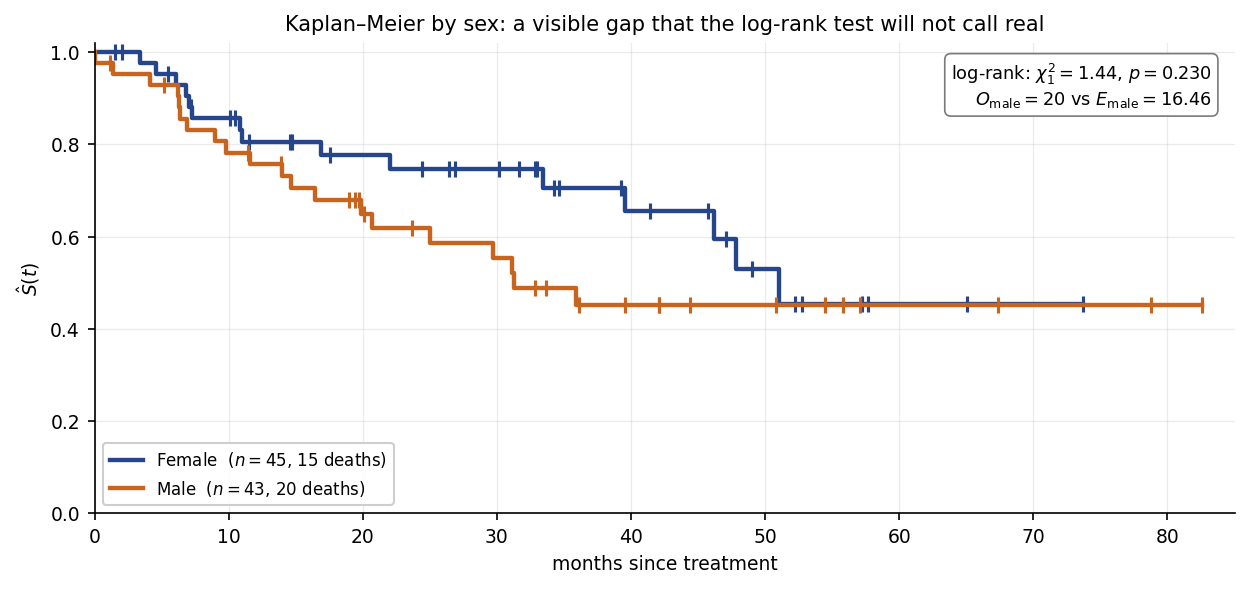
\includegraphics[width=0.9\textwidth,height=0.51\textheight,keepaspectratio]{ch11_km_sex.png}
  \end{center}
  \begin{takeaway}
    The gap looks real: medians $31.25$ (men) against $51.02$ months (women), and
    $\hat S(30)=0.553$ against $0.747$. But the bands overlap throughout. We need a test
    that compares the \emph{whole curves} while respecting the censoring.
  \end{takeaway}
\end{frame}

\begin{frame}{One $2\times2$ table at every death time}
  \footnotesize
  \begin{center}\scriptsize
  \begin{tabular}{l|cc|c}
    \toprule
    At time $t_k$ & Died & Survived & At risk \\
    \midrule
    Group 1 & $d_{1k}$ & $r_{1k}-d_{1k}$ & $r_{1k}$ \\
    Group 2 & $d_{2k}$ & $r_{2k}-d_{2k}$ & $r_{2k}$ \\
    \midrule
    Total & $d_k$ & $r_k-d_k$ & $r_k$ \\
    \bottomrule
  \end{tabular}
  \end{center}
  \begin{readme}[The null hypothesis table by table]
    Under $H_0: S_1(t)=S_2(t)$ the $d_k$ deaths at $t_k$ are allocated purely by how many
    are at risk, so, conditioning on the margins,
    \[
      E_{1k}=d_k\,\frac{r_{1k}}{r_k},
      \qquad
      V_{1k}=\frac{d_k\,(r_{1k}/r_k)\,(1-r_{1k}/r_k)\,(r_k-d_k)}{r_k-1}.
    \]
    ($E_{1k}$ and $V_{1k}$ are the hypergeometric mean and variance of $d_{1k}$.)
  \end{readme}
  \begin{takeaway}
    Censoring enters only through $r_{1k}$ and $r_{2k}$, exactly as in Kaplan--Meier: a
    sequence of small fair-allocation checks, then one sum.
  \end{takeaway}
\end{frame}

\begin{frame}{The log-rank statistic}
  \scriptsize
  \begin{block}{Rule}
    Accumulate over all $K$ death times, then standardise:
    \[
      \boxed{\;
        Z=\frac{O_1-E_1}{\sqrt{V_1}}
         =\frac{\sum_{k=1}^{K}\bigl(d_{1k}-E_{1k}\bigr)}{\sqrt{\sum_{k=1}^{K}V_{1k}}},
        \qquad Z^2 \stackrel{H_0}{\approx} \chi^2_1 .\;}
    \]
  \end{block}
  \begin{readme}
    \begin{itemize}
      \item $O_1=\sum_k d_{1k}$: deaths actually seen in group 1; $E_1=\sum_k E_{1k}$: the
            deaths group 1 would get if the groups were identical.
      \item $Z>0$ means group 1 died \emph{more} than its share of the risk sets warranted.
            Report $Z^2$ against $\chi^2_1$, or $Z$ against $N(0,1)$ for a direction.
      \item Adding the tables, rather than pooling the data once, is what keeps the
            comparison valid under censoring.
    \end{itemize}
  \end{readme}
  \begin{takeaway}
    The log-rank test is the observed-minus-expected count of events, scaled by
    its own standard error. Nothing is assumed about the shape of $S$.
  \end{takeaway}
\end{frame}

\begin{frame}{BrainCancer by sex: the real numbers}
  \footnotesize
  \begin{numexample}[Accumulating over all $35$ death times]
    \[
      O_{\text{male}}=20,\qquad
      E_{\text{male}}=16.4605,\qquad
      V_{\text{male}}=8.6969 ,
    \]
    \[
      Z=\frac{20-16.4605}{\sqrt{8.6969}}=\frac{3.5395}{2.9491}=1.200,
      \qquad
      Z^2=\chi^2_1=1.4405,
      \qquad p=0.230 .
    \]
    Men suffered $3.54$ more deaths than their share of the risk sets predicts --- a real
    but unremarkable excess, about $1.2$ standard errors.
  \end{numexample}
  \begin{takeaway}
    $p=0.230$: with $88$ patients and $35$ deaths there is \textbf{no evidence} of a sex
    difference in survival. A visible gap between two curves and a $20$-month gap between
    medians is entirely consistent with chance at this sample size.
  \end{takeaway}
  \begin{industry}[Clinical development: powering on events rather than patients]
  \scriptsize
    The precision of a log-rank test is governed by $V_1$, which grows with the number of
    \emph{events}. Trials are therefore sized in events, and event-driven analyses are
    triggered when the count is reached --- recruiting more patients into a low-event
    setting buys surprisingly little power.
  \end{industry}
\end{frame}


\begin{frame}{The log-rank arithmetic, drawn}
  \begin{center}
    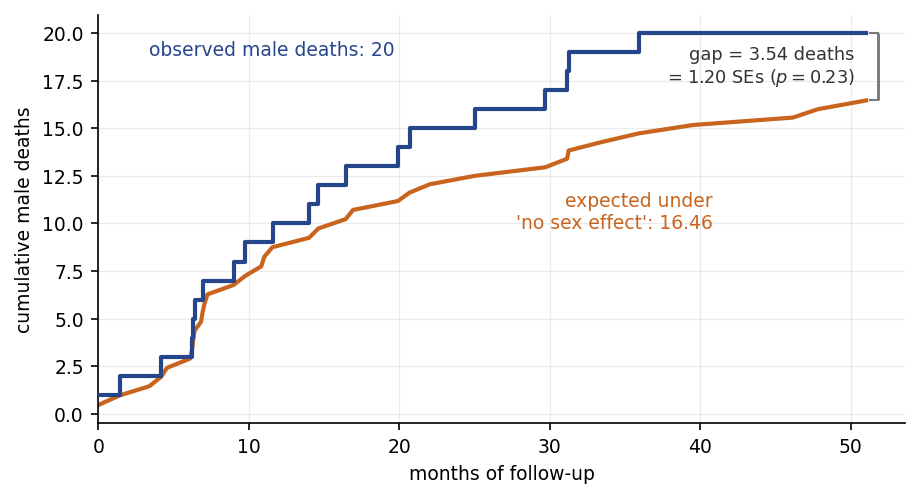
\includegraphics[width=0.68\textwidth,height=0.50\textheight,keepaspectratio]{ch11_logrank_oe.png}
  \end{center}
  \begin{takeaway}
    The previous slide's sum, accumulated over the death times: observed male
    deaths step to $O = 20$, the no-effect track climbs to $E = 16.46$. The
    $3.54$-death gap is $1.20$ standard errors --- two curves that never
    really separate ($p = 0.23$).
  \end{takeaway}
\end{frame}

\begin{frame}{What the log-rank test cannot see}
  \begin{center}
    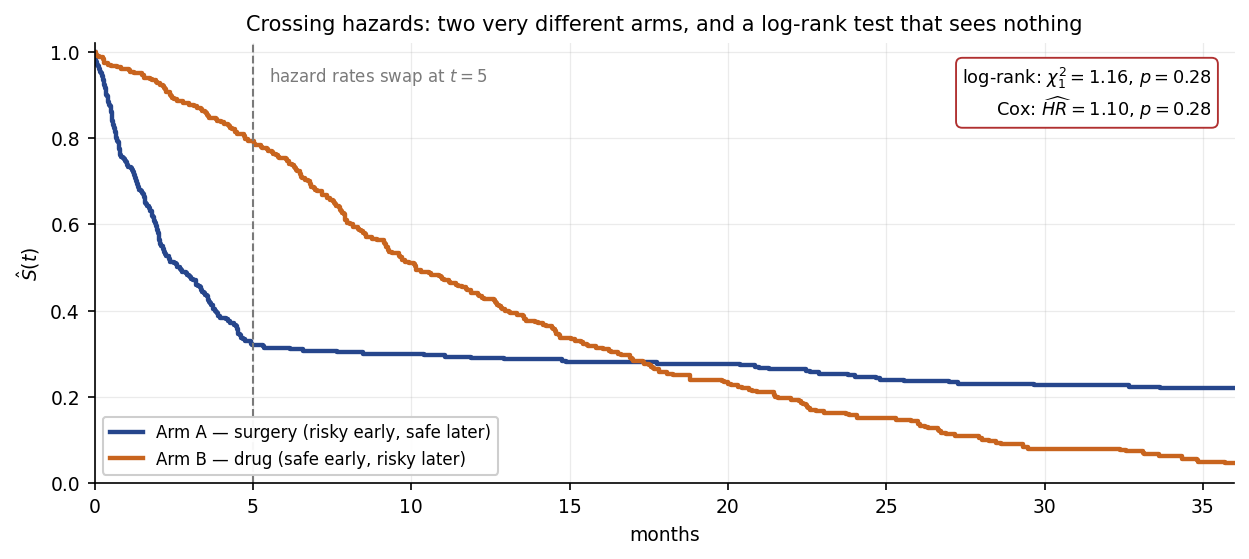
\includegraphics[width=0.88\textwidth,height=0.5\textheight,keepaspectratio]{ch11_crossing.png}
  \end{center}
  \begin{mistake}[A large $p$-value is not ``the arms are the same'']
    Simulated trial, $300$ per arm: surgery is dangerous early and safe later, the drug is
    the reverse. At $6$ months $\hat S_A=0.313$ against $\hat S_B=0.753$; at $36$ months
    the ranking has reversed, $0.220$ against $0.047$. The log-rank statistic is
    $\chi^2_1=1.16$, $p=0.28$: the early and late excesses \textbf{cancel in the sum}
    $O_1-E_1$. Plot first, test second --- and when curves cross, compare at fixed
    horizons or by RMST instead.
  \end{mistake}
\end{frame}

% ------------------------------------------------------------
\begin{frame}{Exercise 11.4 --- The log-rank test by hand [Math]}
\begin{exercise}
  Two treatment arms, times in months ($^{+}$ = censored):
  \[
    \text{A: } 6,\; 7^{+},\; 10,\; 15^{+}
    \qquad\qquad
    \text{B: } 3,\; 5,\; 9,\; 12^{+}
  \]
  \begin{enumerate}
    \item List the death times and, at each, the numbers at risk $r_{Ak}$, $r_{Bk}$.
    \item Compute $O_A$ and $E_A=\sum_k d_k r_{Ak}/r_k$.
    \item Given $V_A=1.1893$, compute the log-rank statistic and compare it with
          $\chi^2_1$ (the $5\%$ critical value is $3.84$).
    \item State the conclusion, and one reason it should not surprise you.
  \end{enumerate}
\end{exercise}
\end{frame}

\begin{frame}{Solution --- Exercise 11.4}
  \scriptsize
\begin{solutionbox}
  \tiny
  \textbf{Parts 1--2 --- the table.} Death times are $3,5,6,9,10$ (censorings are not
  death times, but they do leave the risk sets):
  \[
    \begin{array}{c|c|c|c|c|c|c}
      t_k & r_{Ak} & r_{Bk} & r_k & d_k & d_{Ak} & E_{Ak}=d_k r_{Ak}/r_k\\ \hline
      3  & 4 & 4 & 8 & 1 & 0 & 0.5000\\
      5  & 4 & 3 & 7 & 1 & 0 & 0.5714\\
      6  & 4 & 2 & 6 & 1 & 1 & 0.6667\\
      9  & 2 & 2 & 4 & 1 & 0 & 0.5000\\
      10 & 2 & 1 & 3 & 1 & 1 & 0.6667\\ \hline
         &   &   &   &   & O_A=2 & E_A=2.9048
    \end{array}
  \]
  At $t=5$, arm A still has all four subjects at risk while B is down to $\{5,9,12\}$;
  by $t=9$ arm A is $\{10,15\}$ because $6$ died and $7^{+}$ was censored.

  \medskip
  \textbf{Part 3 --- the statistic.}
  \[
    Z=\frac{2-2.9048}{\sqrt{1.1893}}=\frac{-0.9048}{1.0906}=-0.830,
    \qquad Z^2=0.688 < 3.84,\qquad p=0.407 .
  \]
  \textbf{Part 4 --- conclusion.} No evidence of a difference. Arm A had \emph{fewer}
  deaths than expected ($Z<0$), but with only five events the standard error swamps the
  gap: $V_A$ grows with events, and five is not a study.
\end{solutionbox}
\begin{mistake}
  \scriptsize
  Building the tables at censoring times. Only death times contribute a term; a censoring
  merely shrinks $r_{Ak}$ or $r_{Bk}$ for later tables.
\end{mistake}
\end{frame}

% ============================================================
\section{Cox Model}
% ============================================================

\begin{frame}{From two curves to many covariates: the hazard}
  \scriptsize
  Comparing curves group by group does not scale to \texttt{ki}, \texttt{gtv},
  \texttt{diagnosis}, \dots\ We need a regression --- and it is built on the hazard.
  \begin{block}{Definition}
    \[
      \boxed{\;h(t)=\lim_{\Delta\to 0}
        \frac{\Pr\bigl(t< T\le t+\Delta \mid T>t\bigr)}{\Delta}\;}
    \]
  \end{block}
  \begin{readme}
    \begin{itemize}
      \item A \textbf{rate}, not a probability: events per unit time \emph{among those
            still at risk}. It can exceed $1$ and has units $1/\text{time}$.
      \item ``Given that you have survived to $t$, how fast is the event arriving right
            now?'' --- the natural quantity for censored data, because it conditions on
            exactly the set we can still observe.
      \item Cumulative hazard $H(t)=\int_0^t h(u)du$ ties it back to survival:
            $S(t)=e^{-H(t)}$, and equivalently $h(t)=-\frac{d}{dt}\log S(t)$.
      \item So $h$, $H$ and $S$ are three views of one object: fix any one and the others
            follow.
    \end{itemize}
  \end{readme}
  \begin{takeaway}
    Model the hazard and you have modelled the survival curve --- with the censoring
    handled for free.
  \end{takeaway}
\end{frame}

\begin{frame}{The Cox proportional-hazards model}
  \scriptsize
  \begin{block}{Model}
    \[
      \boxed{\;h(t\mid x_i)=h_0(t)\,\exp\bigl(x_i^{\top}\beta\bigr)
        =h_0(t)\exp\bigl(\beta_1x_{i1}+\cdots+\beta_px_{ip}\bigr)\;}
    \]
  \end{block}
  \begin{readme}
    \begin{itemize}
      \item $h_0(t)$: the \textbf{baseline hazard}, shared by everyone and left completely
            unspecified --- any non-negative function of time.
      \item $\exp(x_i^{\top}\beta)$: a subject-specific multiplier, constant in $t$ and
            positive whatever $\beta$ is. There is no intercept: it would be absorbed
            into $h_0$.
      \item \textbf{Semi-parametric}: non-parametric in time, parametric in the covariates.
      \item ``Proportional'': for two subjects the hazard \emph{ratio}
            $\exp\{(x_i-x_j)^{\top}\beta\}$ does not depend on $t$ --- the curves may have
            any shape, but the vertical factor between them never changes.
    \end{itemize}
  \end{readme}
  \begin{takeaway}
    All the flexibility goes into time, all the interpretation into $\beta$. That
    division of labour is why this model has dominated applied survival analysis
    since 1972.
  \end{takeaway}
\end{frame}

\begin{frame}{What ``proportional hazards'' looks like}
  \begin{center}
    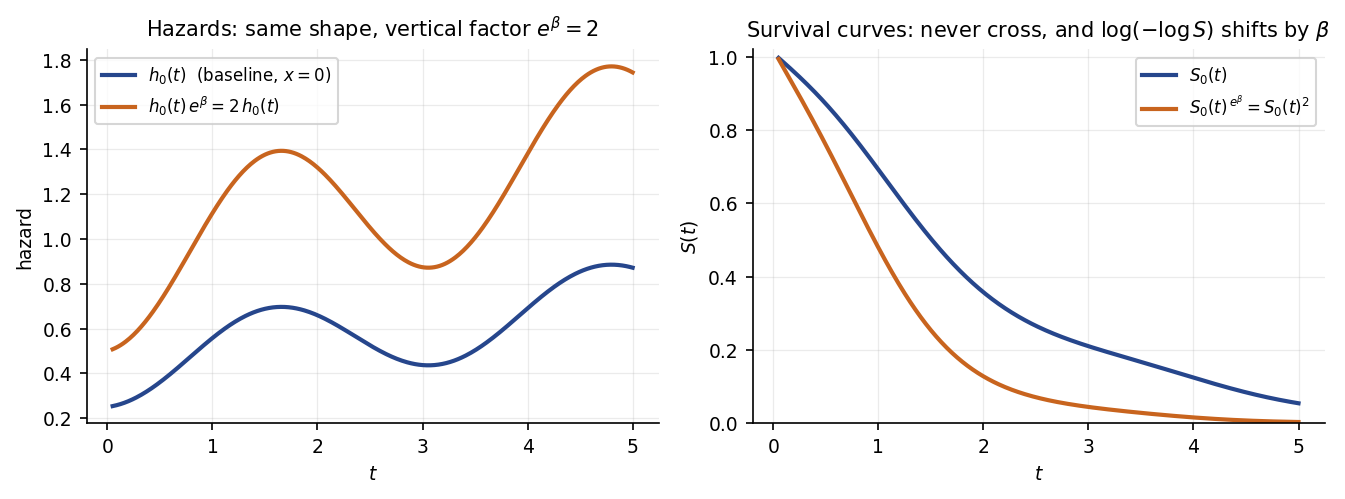
\includegraphics[width=0.94\textwidth,height=0.5\textheight,keepaspectratio]{ch11_ph.png}
  \end{center}
  \begin{takeaway}
    Left: the baseline hazard may wiggle as much as it likes; the covariate only
    multiplies it, here by $e^{\beta}=2$. Right: the survival curves are then
    $S_0(t)$ and $S_0(t)^{2}$ --- they \textbf{cannot cross}, and
    $\log(-\log S)$ shifts by the constant $\beta$. Both are testable consequences.
  \end{takeaway}
\end{frame}

\begin{frame}{Estimating $\beta$ without ever estimating $h_0$}
  \scriptsize
  \begin{block}{The partial likelihood (Cox, 1972)}
    \[
      \boxed{\;
        \mathrm{PL}(\beta)=\prod_{i:\,\delta_i=1}
        \frac{\exp(x_i^{\top}\beta)}
             {\sum_{j\in R(Y_i)}\exp(x_j^{\top}\beta)}\;}
      \qquad R(Y_i)=\{j: Y_j\ge Y_i\}
    \]
  \end{block}
  \begin{readme}[Where the baseline went]
    \begin{itemize}
      \item At each observed death ask: \emph{among everyone still at risk, what was the
            chance that this subject was the one to die?} That chance is
            $h_0(Y_i)e^{x_i^\top\beta}\big/\sum_{j\in R(Y_i)}h_0(Y_i)e^{x_j^\top\beta}$,
            and $h_0(Y_i)$ is in every term of numerator and denominator, so it
            \textbf{cancels exactly}.
      \item Maximise $\log \mathrm{PL}$ numerically; $\hat\beta$ is consistent and
            asymptotically normal, with the usual Wald and likelihood-ratio tests. Censored
            subjects contribute no factor but populate the risk sets of earlier deaths.
      \item \textbf{Buys:} no distribution for $T$; only the \emph{order} of the times
            matters. \textbf{Costs:} no absolute risk from $\hat\beta$ alone.
    \end{itemize}
  \end{readme}
  \begin{industry}[Credit risk: why ordering-only matters]
    A prepayment model fitted on loan age transfers to a book measured in payment counts,
    because the partial likelihood uses only who-was-at-risk-when.
  \end{industry}
\end{frame}

\begin{frame}{Coefficients are log hazard ratios}
  \scriptsize
  \begin{block}{Reading rule}
    \[
      \boxed{\;
        \frac{h(t\mid x_j+1)}{h(t\mid x_j)}=e^{\beta_j}
        \quad\text{for every } t
        \qquad\Longrightarrow\qquad
        \beta_j=\log \mathrm{HR}_j . \;}
    \]
  \end{block}
  \begin{readme}
    \begin{itemize}
      \item $e^{\beta_j}>1$: higher $x_j$ means a \emph{higher} event rate, so shorter
            survival. $e^{\beta_j}<1$: protective. $e^{\beta_j}=1$: no effect.
      \item A $c$-unit change multiplies the hazard by $e^{c\beta_j}$ --- choose $c$ so
            the number is clinically meaningful (ten Karnofsky points, not one).
      \item Confidence intervals are computed on the $\beta$ scale and then exponentiated,
            which is why hazard-ratio intervals are asymmetric around $e^{\hat\beta_j}$.
      \item Test $H_0:\beta_j=0$ (i.e.\ $\mathrm{HR}=1$) with $z=\hat\beta_j/
            \mathrm{se}(\hat\beta_j)$.
    \end{itemize}
  \end{readme}
  \begin{takeaway}
    One number per covariate, valid at all times --- the payoff of the
    proportional-hazards assumption, and the reason it must be checked.
  \end{takeaway}
\end{frame}

\begin{frame}{The fitted model on BrainCancer}
  \footnotesize
  \begin{center}
  \begin{tabular}{@{}lrrrrl@{}}
    \toprule
    \textbf{Covariate} & $\hat\beta$ & $\mathrm{se}$ & $e^{\hat\beta}$ &
    \textbf{$95\%$ CI for} $e^{\hat\beta}$ & $p$ \\
    \midrule
    \texttt{ki} (per point)            & $-0.0550$ & $0.0183$ & $0.947$ & $[0.913,\ 0.981]$ & $0.003$ \\
    \texttt{gtv} (per cm$^3$)          & $\ \ 0.0343$ & $0.0223$ & $1.035$ & $[0.991,\ 1.081]$ & $0.125$ \\
    \texttt{sex} Male                  & $\ \ 0.1837$ & $0.3604$ & $1.202$ & $[0.593,\ 2.435]$ & $0.610$ \\
    \texttt{diagnosis} HG glioma       & $\ \ 2.1546$ & $0.4505$ & $8.624$ & $[3.566,\ 20.855]$ & $<0.001$ \\
    \texttt{diagnosis} LG glioma       & $\ \ 0.9150$ & $0.6382$ & $2.497$ & $[0.715,\ 8.722]$ & $0.152$ \\
    \texttt{diagnosis} Other           & $\ \ 0.8857$ & $0.6579$ & $2.425$ & $[0.668,\ 8.803]$ & $0.178$ \\
    \texttt{loc} Supratentorial        & $\ \ 0.4412$ & $0.7037$ & $1.555$ & $[0.391,\ 6.174]$ & $0.531$ \\
    \texttt{stereo} SRT                & $\ \ 0.1778$ & $0.6016$ & $1.195$ & $[0.367,\ 3.884]$ & $0.768$ \\
    \bottomrule
  \end{tabular}
  \end{center}
  \begin{readme}[Housekeeping before interpretation]
    $n=87$ complete cases, $35$ deaths. \texttt{diagnosis} is coded against
    \textbf{Meningioma}; every diagnosis row is a comparison with that group. Overall
    likelihood-ratio test: $\chi^2_8=41.4$, $p=1.8\times10^{-6}$ --- the covariates
    together matter, even though most individually do not.
  \end{readme}
\end{frame}

\begin{frame}{Reading two coefficients out loud}
  \footnotesize
  \begin{numexample}[Karnofsky index and a diagnosis]
    \textbf{\texttt{ki}:} $\hat\beta=-0.0550$, so one extra Karnofsky point multiplies the
    death rate by $e^{-0.0550}=0.947$ --- a $5.3\%$ reduction. Per unit is too fine to
    discuss, so rescale:
    \[
      e^{10\times(-0.0550)}=e^{-0.550}=0.577 .
    \]
    \emph{``Holding tumour type, volume, site, sex and technique fixed, ten more Karnofsky
    points are associated with a $42\%$ lower death rate at every follow-up time.''}
    \medskip
    \textbf{HG glioma vs.\ meningioma:} $e^{2.1546}=8.62$, CI $[3.57,\ 20.86]$. The death
    rate is $8.6$ times higher, and even the optimistic end of the interval is a
    $3.6$-fold increase. In survival terms at $\texttt{ki}=80$: $\hat S(24)=0.874$ for
    meningioma against $0.314$ for HG glioma.
  \end{numexample}
  \begin{takeaway}
    Always name the comparison, the units, and the phrase ``holding the other
    covariates fixed''. A hazard ratio without its reference level is not a result.
  \end{takeaway}
\end{frame}

\begin{frame}{A hazard ratio is not a risk ratio}
  \begin{mistake}[Three different quantities that students merge into one]
    \begin{itemize}
      \item \textbf{Hazard ratio} $e^{\beta}$: ratio of \emph{instantaneous rates} among
            those still at risk, at a given time. It is a ratio of \emph{speeds}.
      \item \textbf{Risk ratio} $\frac{1-S_1(t)}{1-S_2(t)}$: ratio of cumulative
            probabilities by a \emph{fixed} time $t$. It depends on $t$ and is always
            closer to $1$ than the hazard ratio.
      \item \textbf{Odds ratio} $\frac{p_1/(1-p_1)}{p_2/(1-p_2)}$: from logistic
            regression, on the odds scale, ignoring time entirely.
    \end{itemize}
    ``$\mathrm{HR}=8.6$'' does \textbf{not} mean HG glioma patients are $8.6$ times more
    likely to die, nor that they die $8.6$ times sooner. At $24$ months the actual risk
    ratio here is $(1-0.314)/(1-0.874)=5.4$, and by $36$ months it is $4.3$ --- the same
    constant hazard ratio produces a shrinking risk ratio.
  \end{mistake}
  \begin{takeaway}
    Report a hazard ratio for the mechanism and a survival probability at a stated
    horizon for the decision. Never translate one into the other by intuition.
  \end{takeaway}
\end{frame}

% ------------------------------------------------------------
\begin{frame}{Exercise 11.5 --- Hazard-ratio arithmetic [Math]}
\begin{exercise}
  A Cox model for time to churn is fitted with covariates
  \texttt{monthly\_price} (in euros) and \texttt{onboarded} ($1$ = completed onboarding):
  \[
    \hat\beta_{\text{price}}=0.024\ (\mathrm{se}\ 0.006),
    \qquad
    \hat\beta_{\text{onboarded}}=-0.693\ (\mathrm{se}\ 0.210).
  \]
  \begin{enumerate}
    \item Give the hazard ratio for a $10$-euro price increase.
    \item Give the hazard ratio for completing onboarding, and interpret it in one
          sentence.
    \item Test $H_0:\beta_{\text{onboarded}}=0$ and give a $95\%$ interval for its
          hazard ratio.
    \item Two customers differ by $20$ euros in price, and the cheaper one completed
          onboarding. What is their hazard ratio?
  \end{enumerate}
\end{exercise}
\end{frame}

\begin{frame}{Solution --- Exercise 11.5}
\begin{solutionbox}
  \scriptsize
  \textbf{Part 1 --- rescaling.} A $c$-unit change multiplies the hazard by $e^{c\beta}$, so
  $e^{10\times 0.024}=e^{0.24}=1.271$: a $27.1\%$ higher churn rate per $10$ euros.

  \medskip
  \textbf{Part 2 --- a binary covariate.} $e^{-0.693}=0.500$. Onboarded customers churn at
  \emph{half} the rate of comparable customers who did not onboard, at every tenure.

  \medskip
  \textbf{Part 3 --- test and interval.} $z=-0.693/0.210=-3.30$, so $p\approx0.001$: clear
  evidence. Build the interval on the $\beta$ scale, \emph{then} exponentiate:
  $-0.693 \pm 1.96(0.210)=[-1.105,-0.281]$, so the hazard-ratio interval is
  $[e^{-1.105},e^{-0.281}]=[0.331,0.755]$ --- asymmetric around $0.500$, as every
  hazard-ratio interval is.

  \medskip
  \textbf{Part 4 --- combining covariates.} Hazards multiply, so log hazards add; with the
  expensive, non-onboarded customer as the numerator,
  $e^{20(0.024)}/e^{-0.693}=e^{1.173}=3.23$.
\end{solutionbox}
\begin{mistake}
  \scriptsize
  Averaging the two hazard ratios, or exponentiating after adding standard errors.
  Combine on the \emph{log} scale, exponentiate once at the end.
\end{mistake}
\end{frame}

% ============================================================
\section{Practice}
% ============================================================

\begin{frame}{Proportional hazards is an assumption, not a result}
  \footnotesize
  \begin{readme}[Two checks --- one formal and one visual]
    \begin{itemize}
      \item \textbf{Schoenfeld residuals.} If $\mathrm{HR}$ is constant, the residuals for
            covariate $j$ show \emph{no trend in time}. Test the correlation between the
            residuals and (a transform of) time: a small $p$-value is evidence
            \emph{against} proportionality.
      \item \textbf{Complementary log-log plot.} Under PH the curves
            $\log(-\log\hat S(t))$ for two strata differ by the constant $\beta$, so they
            should look \textbf{parallel} --- crossing or converging curves are a warning.
    \end{itemize}
  \end{readme}
  \begin{numexample}[Schoenfeld test on all eight BrainCancer covariates]
    Every $p$-value exceeds $0.39$ (\texttt{ki} $0.82$, HG glioma $0.82$, \texttt{gtv} $0.48$;
    the smallest is $0.40$, for \texttt{sex}). \textbf{No evidence against} proportional hazards --- which
    with $35$ events is a weak reassurance, not a clean bill of health.
  \end{numexample}
  \begin{mistake}
  \scriptsize
    Reading ``$p=0.82$'' as ``proportional hazards holds''. Failing to reject is not
    accepting; with few events these tests have very little power.
  \end{mistake}
\end{frame}

\begin{frame}{When proportional hazards fails: five honest options}
  \footnotesize
  \begin{readme}[In rough order of how much you give up]
    \begin{enumerate}
      \item \textbf{Stratify} on the offending variable: fit
            $h(t\mid x)=h_{0g}(t)e^{x^\top\beta}$ with a separate baseline per stratum.
            You lose its coefficient, and keep everything else.
      \item \textbf{Interact with time}: let $\beta_j(t)=\beta_j+\gamma_j\log t$, and
            report an early and a late hazard ratio.
      \item \textbf{Split the follow-up} into periods and fit a hazard ratio in each ---
            the crude version of the same idea, and easy to explain.
      \item \textbf{Change the target}: compare $\hat S$ at pre-specified horizons, or
            compare $\mathrm{RMST}(\tau)$. No proportionality needed at all.
      \item \textbf{Use an accelerated-failure-time model} (Weibull, log-logistic), which
            multiplies \emph{time} rather than the hazard.
    \end{enumerate}
  \end{readme}
  \begin{takeaway}
    A crossing-hazards problem is a \emph{question} problem: ``is A better than B?''
    has no time-free answer, so pick the horizon that matters to the decision and
    report the comparison there.
  \end{takeaway}
\end{frame}

\begin{frame}{From coefficients to a curve for one subject}
  \footnotesize
  \begin{center}
    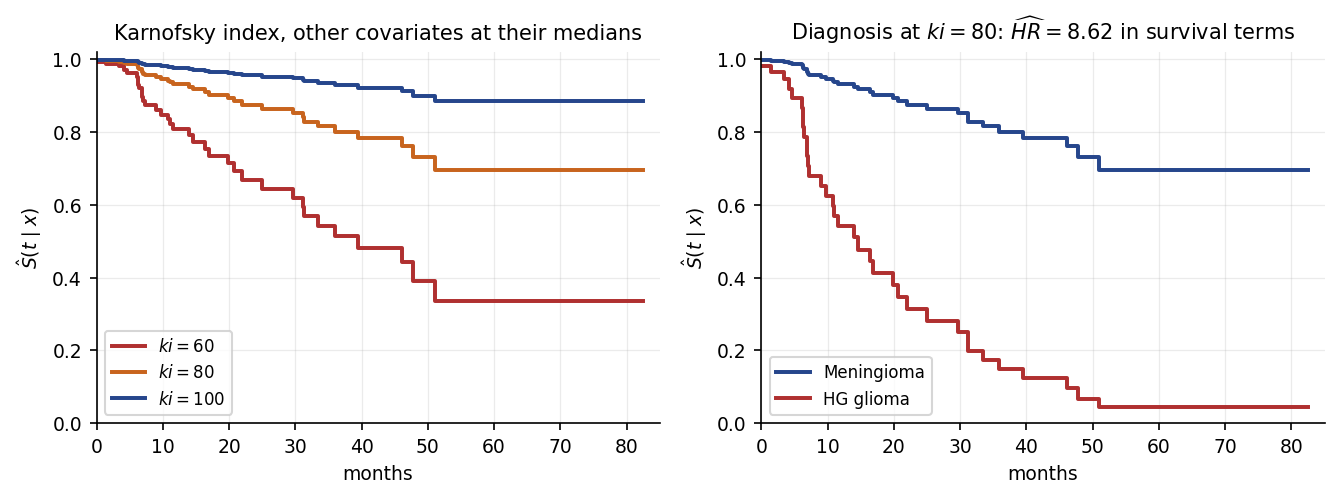
\includegraphics[width=0.94\textwidth,height=0.5\textheight,keepaspectratio]{ch11_predict.png}
  \end{center}
  \begin{takeaway}
    Combining $\hat\beta$ with Breslow's baseline gives
    $\hat S(t\mid x)=\hat S_0(t)^{\exp(x^\top\hat\beta)}$. At $36$ months, with the other
    covariates at their medians, $\hat S=0.514$ for $\texttt{ki}=60$ against $0.801$ at
    $80$ and $0.929$ at $100$; the median is $39.5$ months at $\texttt{ki}=60$ and is
    never reached above that. This is the form in which a clinician or a pricing team can
    use the model.
  \end{takeaway}
\end{frame}

\begin{frame}{Evaluating a survival model}
  \scriptsize
  \begin{block}{Harrell's concordance index}
    \[
      C=\Pr\bigl(\hat\eta_i>\hat\eta_j \;\big|\; T_i<T_j\bigr),
      \qquad \hat\eta_i=x_i^{\top}\hat\beta ,
    \]
    estimated over all \emph{comparable} pairs --- those whose ordering censoring lets us
    determine.
  \end{block}
  \begin{readme}
    \begin{itemize}
      \item The survival analogue of the AUC: $0.5$ is random ordering, $1.0$ is perfect
            ranking. The BrainCancer fit reaches $C=0.794$.
      \item It grades the \emph{ranking} of risks only --- a model can have $C=0.79$ and
            still predict badly calibrated survival probabilities.
      \item So pair it with calibration --- bucket subjects by $\hat\eta$ and overlay the
            predicted curve on each bucket's Kaplan--Meier curve --- and cross-validate,
            exactly as in Chapter 5: read on the training data, $C$ is optimistic.
    \end{itemize}
  \end{readme}
  \begin{industry}[Model risk: the two questions a validator asks]
    \emph{Discrimination} --- does it rank? (C-index, cross-validated.) \emph{Calibration}
    --- are the probabilities right at the horizons the business uses? A provisioning model
    fails validation on the second even when it passes the first.
  \end{industry}
\end{frame}

\begin{frame}{High-dimensional survival: the regularised Cox model}
  \footnotesize
  \begin{block}{Penalised partial likelihood}
    \[
      \max_{\beta}\ \Bigl\{\log \mathrm{PL}(\beta)
        \;-\;\lambda\bigl[(1-\alpha)\tfrac12\|\beta\|_2^2+\alpha\|\beta\|_1\bigr]\Bigr\}
    \]
  \end{block}
  \begin{readme}[Chapter 6 transplanted]
    \begin{itemize}
      \item With $p>n$ --- $20\,000$ genes and $200$ patients --- the partial likelihood
            has no unique maximum and $\hat\beta$ does not exist. Exactly the Chapter 6
            situation, one likelihood along.
      \item $\alpha=1$ gives the \textbf{lasso}-Cox (a sparse risk score); $\alpha=0$ the
            ridge-Cox; in between, the elastic net. Choose $\lambda$ by cross-validating
            the partial likelihood, \emph{not} the C-index alone.
      \item The resulting linear predictor $x^\top\hat\beta$ is the risk score behind
            commercial genomic assays.
    \end{itemize}
  \end{readme}
  \begin{industry}[Oncology diagnostics: from a signature to a decision]
  \scriptsize
    A lasso-Cox on gene expression yields a handful of genes and one score; the score is
    then dichotomised at a threshold chosen on \emph{clinical} grounds and validated on an
    independent cohort. Sparsity is what makes the assay cheap enough to run.
  \end{industry}
\end{frame}

% ------------------------------------------------------------
\begin{frame}{Exercise 11.6 --- Diagnosing and fixing a PH violation [Concept]}
\begin{exercise}
  A retention team fits a Cox model for time to churn. The Schoenfeld test for the
  covariate \texttt{annual\_contract} returns $p=0.002$; its complementary log-log curves
  cross at about month $14$. The estimated hazard ratio is $0.98$ with $p=0.81$.
  \begin{enumerate}
    \item What is the substantive story behind crossing curves here?
    \item Explain why $\mathrm{HR}=0.98$, $p=0.81$ is not evidence that contract type
          does not matter.
    \item Propose two concrete fixes and state what each costs.
    \item The team must publish a single number for the next board meeting. What do you
          recommend?
  \end{enumerate}
\end{exercise}
\end{frame}

\begin{frame}{Solution --- Exercise 11.6}
  \footnotesize
\begin{solutionbox}
  \scriptsize
  \textbf{Part 1 --- the story.} Annual contracts lock customers in, so their hazard is
  very low early and then spikes at renewal; monthly customers churn at a steady moderate
  rate. Before month $14$ annual is protective, afterwards it is dangerous. That is a
  time-varying hazard ratio, i.e.\ a PH violation, and the crossing is not a nuisance ---
  it \emph{is} the finding.

  \medskip
  \textbf{Part 2 --- why the null result is an artefact.} A single $\beta$ forces one
  constant hazard ratio, and the fit lands near the time-average of a
  protective-then-harmful effect. Early and late excesses cancel, so
  $\hat\beta\approx0$ --- the same cancellation that made the log-rank test blind to
  crossing curves. The model was asked the wrong question and answered it faithfully.

  \medskip
  \textbf{Part 3 --- two fixes.}
  \begin{itemize}
    \item \textbf{Split the follow-up} at month $14$ and fit a hazard ratio in each
          period. Cost: the split point is a choice, and choosing it from these data
          invalidates the naive $p$-values.
    \item \textbf{Stratify} on \texttt{annual\_contract}: every other coefficient stays
          interpretable and the baselines are free to differ. Cost: you get no hazard
          ratio for contract type at all.
  \end{itemize}
  \medskip
  \textbf{Part 4 --- the board number.} Not a hazard ratio. Quote retention at a
  decision-relevant horizon --- $\hat S(12)$ and $\hat S(24)$ by contract type with
  intervals --- or $\mathrm{RMST}(24)$. Both are well defined when hazards cross.
\end{solutionbox}
\end{frame}

% ------------------------------------------------------------
\begin{frame}{Extended Exercise 11.2 --- The Cox model in Python [Python]}
\begin{longexercise}
  Using \texttt{BrainCancer} and \texttt{lifelines}:
  \begin{enumerate}
    \item Fit a Cox model with all six covariates, coding \texttt{diagnosis} against
          \textbf{Meningioma}. Report $\hat\beta$, $e^{\hat\beta}$ and $p$ for
          \texttt{ki} and for HG glioma.
    \item Convert the \texttt{ki} coefficient into a hazard ratio for a ten-point
          increase, and write the one-sentence interpretation.
    \item Report the concordance index, and the overall likelihood-ratio test.
    \item Test proportional hazards with Schoenfeld residuals and state the conclusion.
    \item Predict and plot $\hat S(t\mid x)$ for $\texttt{ki}\in\{60,80,100\}$ with the
          other covariates at their medians.
  \end{enumerate}
\end{longexercise}
\begin{labnote}[Run this live]
  The worked solution sits in \texttt{chapter\_11\_lab.ipynb} under
  \emph{Lecture exercises --- worked Python solutions}: the cell headed
  \emph{Extended Exercise 11.2 --- The Cox model in Python [Python]}.
\end{labnote}
\end{frame}

\begin{frame}[fragile]{Solution --- Extended Exercise 11.2 (1/2)}
\begin{solutionbox}[Solution --- code]
\begin{lstlisting}[basicstyle=\ttfamily\scriptsize]
import numpy as np, pandas as pd
from lifelines import CoxPHFitter
from lifelines.statistics import proportional_hazard_test
BC = load('BrainCancer', index_col=0).dropna()        # 87 complete cases
BC['diagnosis'] = pd.Categorical(BC['diagnosis'],     # Meningioma = reference
        categories=['Meningioma', 'HG glioma', 'LG glioma', 'Other'])
X = pd.get_dummies(BC, drop_first=True).astype(float) # drop the reference level
cph = CoxPHFitter().fit(X, duration_col='time', event_col='status')
print(cph.summary[['coef', 'exp(coef)', 'p']].round(4))  # log HR, HR, p-value
print('HR per 10 ki : %.3f' % np.exp(10 * cph.params_['ki']))   # rescaled HR
print('C-index      : %.3f' % cph.concordance_index_)           # discrimination
print(proportional_hazard_test(cph, X, time_transform='rank').summary['p'])
med = X.drop(columns=['time','status']).median().to_frame().T   # median profile
prof = pd.concat([med] * 3, ignore_index=True)        # three copies of it
prof['ki'] = [60., 80., 100.]                         # vary one covariate only
cph.predict_survival_function(prof).plot()            # S(t | x) per profile
\end{lstlisting}
\end{solutionbox}
\end{frame}

\begin{frame}{Solution --- Extended Exercise 11.2 (2/2)}
\begin{solutionbox}[Solution --- output and reading]
  \begin{itemize}
    \item \textbf{(1)} \texttt{ki}: $\hat\beta=-0.0550$, $e^{\hat\beta}=0.947$,
          $p=0.003$. HG glioma: $\hat\beta=2.1546$, $e^{\hat\beta}=8.624$, $p<0.001$.
          The remaining six covariates all have $p>0.12$.
    \item \textbf{(2)} $e^{10\times(-0.0550)}=e^{-0.550}=0.577$: \emph{``holding tumour
          type, volume, site, sex and technique fixed, ten more Karnofsky points are
          associated with a $42\%$ lower death rate at every follow-up time.''}
    \item \textbf{(3)} $C=0.794$ --- good discrimination, but read on the training data,
          so optimistic. Likelihood-ratio test $\chi^2_8=41.4$,
          $p=1.8\times10^{-6}$: the covariate block clearly carries signal.
    \item \textbf{(4)} Schoenfeld $p$-values run from $0.40$ to $0.82$: no evidence
          against proportional hazards. With $35$ events, that is weak reassurance.
    \item \textbf{(5)} $\hat S(36\mid \texttt{ki})=0.514,\,0.801,\,0.929$ for
          $\texttt{ki}=60,80,100$. Median $39.5$ months at $60$; not reached at $80$ or
          $100$ within the $82.56$ months of follow-up.
  \end{itemize}
  \smallskip
  \textit{Common mistake:} letting \texttt{get\_dummies} pick the reference level
  alphabetically --- here that is HG glioma, and every diagnosis coefficient changes sign
  and meaning while the fit stays identical.
\end{solutionbox}
\end{frame}

% ------------------------------------------------------------
\begin{frame}{Extended Exercise 11.3 --- Publication bias, measured [Integrative]}
\begin{longexercise}
  \texttt{Publication} records the time in months from completion to publication for
  $244$ NHLBI-funded clinical trials; \texttt{status} $=1$ means published, and
  \texttt{posres} $=1$ means the trial found a statistically significant primary result.
  \begin{enumerate}
    \item A log-rank test comparing publication times by \texttt{posres} gives
          $\chi^2_1=0.84$, $p=0.358$. What does that appear to say about publication bias?
    \item A Cox model with \texttt{posres} alone gives $\widehat{\mathrm{HR}}=1.16$,
          $p=0.360$. Adding \texttt{impact}, \texttt{clinend}, \texttt{multi},
          \texttt{sampsize} and \texttt{budget} moves it to
          $\widehat{\mathrm{HR}}=1.77$, $p=0.001$. Explain how one variable can go from
          null to clearly significant.
    \item Which covariate does most of that work, and by what mechanism?
    \item State the conclusion in one sentence a journal editor would understand.
  \end{enumerate}
\end{longexercise}
\end{frame}

\begin{frame}{Solution --- Extended Exercise 11.3 (1/2)}
  \footnotesize
\begin{solutionbox}[Solution --- what the unadjusted comparison hides]
  \scriptsize
  \textbf{Part 1 --- the apparent answer.} Taken alone, $p=0.358$ says trials with and
  without a positive result are published at indistinguishable rates: no evidence of
  publication bias. The two Kaplan--Meier curves are nearly on top of each other
  (medians $23.1$ vs $25.1$ months).
  \medskip
  \begin{center}
    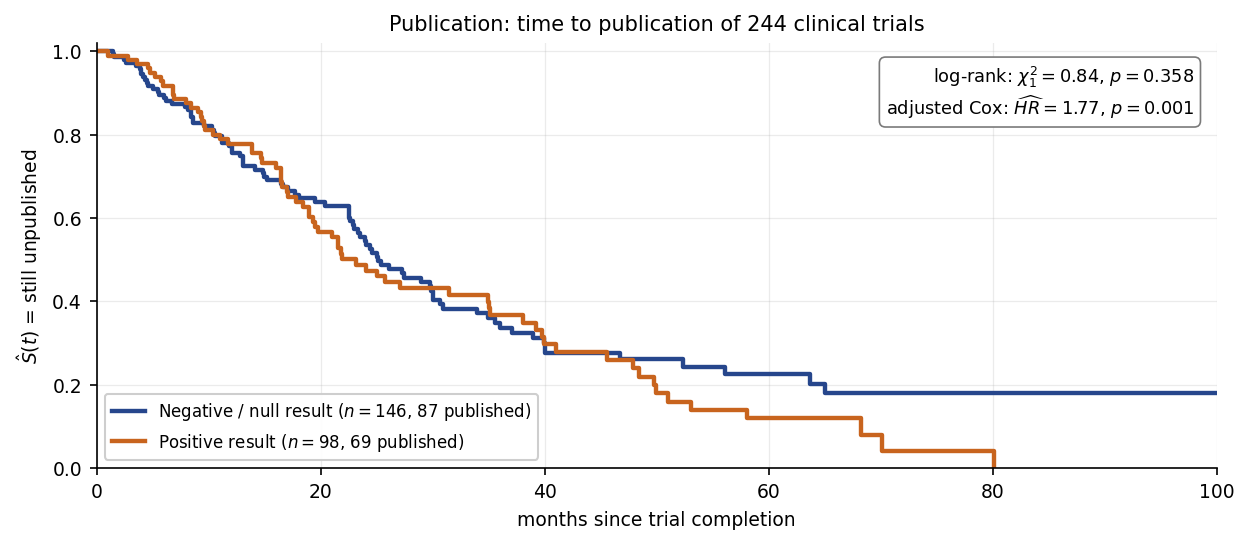
\includegraphics[width=0.72\textwidth,height=0.34\textheight,keepaspectratio]{ch11_x_publication.png}
  \end{center}
  \textbf{Part 2 --- why adjustment changes everything.} The log-rank test is
  \emph{marginal}: it cannot hold anything fixed. \texttt{posres} is entangled with the
  journal-level variables --- and the entanglement works in the opposite direction to the
  effect of interest, masking it. Conditioning on those variables removes the mask, and
  the hazard ratio for publication rises from $1.16$ to $1.77$ ($p=0.001$).
\end{solutionbox}
\end{frame}

\begin{frame}{Solution --- Extended Exercise 11.3 (2/2)}
  \footnotesize
\begin{solutionbox}[Solution --- mechanism and conclusion]
  \scriptsize
  \textbf{Part 3 --- the variable doing the work.} \texttt{impact}, the journal impact
  factor, with $\hat\beta=0.0583$ ($\mathrm{HR}=1.060$ per point, $z=8.7$,
  $p<0.001$) --- by far the strongest term in the model. High-impact journals are slow;
  positive trials aim at them. So a positive result buys a faster \emph{decision} but a
  slower \emph{venue}, and the two effects cancel in the raw comparison.
  \texttt{clinend} (a clinical endpoint) also matters, $\mathrm{HR}=1.73$, $p=0.037$;
  \texttt{multi}, \texttt{sampsize} and \texttt{budget} do not ($p\ge0.075$).

  \medskip
  \textbf{Part 4 --- the sentence.} \emph{``Among comparable trials --- same target
  journal impact, same endpoint type, same size and budget --- those with a positive
  primary result were published at $1.8$ times the rate of those without
  ($p=0.001$), so the raw publication times understate publication bias rather than
  refuting it.''}

  \medskip
  \textbf{The transferable lesson.} A log-rank test answers ``are these two groups
  different?''; a Cox model answers ``is this variable associated with the hazard, given
  the others?''. When those disagree, the covariates --- not the tests --- are telling
  you something.
\end{solutionbox}
\begin{mistake}
  Concluding from $p=0.358$ that publication bias is absent. An unadjusted comparison
  can be null because there is no effect, or because two real effects cancel; only the
  adjusted model distinguishes them.
\end{mistake}
\end{frame}

% ============================================================
\section{Python Lab}
% ============================================================

\begin{frame}{Python lab --- run it live in the notebook}
  \begin{labnote}[Companion notebook: \texttt{chapter\_11\_lab.ipynb}]
    The code in this section is meant to be \textbf{demonstrated live}. Open the companion
    Jupyter notebook and run it cell by cell:
    \begin{itemize}
      \item \S1, \emph{Data and the censoring convention} --- load \texttt{BrainCancer},
            establish that \texttt{status} $=1$ is death;
      \item \S2, \emph{Why the naive analyses fail} --- reproduce the medians
            $11.6$, $23.7$, $47.8$;
      \item \S3, \emph{Kaplan--Meier} --- the curve, its confidence band and the curves
            by sex;
      \item \S4, \emph{Log-rank test}, then \S5, \emph{Cox proportional-hazards model};
      \item \S6, \emph{Checking proportional hazards and predicting curves}.
    \end{itemize}
    Data loads via the \texttt{ISLP} package or the bundled CSV files; the notebook then
    closes with \emph{Lecture exercises --- worked Python solutions} and \S7,
    \emph{Exercises}.
  \end{labnote}
\end{frame}

\begin{frame}[fragile]{Kaplan--Meier and the log-rank test in lifelines}
  \begin{lstlisting}
import pandas as pd                                    # data frames
from lifelines import KaplanMeierFitter                # product-limit fitter
from lifelines.statistics import logrank_test          # two-curve comparison

BC = pd.read_csv('BrainCancer.csv', index_col=0)       # index col = row number
km = KaplanMeierFitter().fit(BC['time'], BC['status']) # status: 1 = death
print('median survival :', km.median_survival_time_)   # 47.8 months

male = BC['sex'] == 'Male'                             # the two groups
res = logrank_test(BC.loc[male, 'time'],   BC.loc[~male, 'time'],
                   BC.loc[male, 'status'], BC.loc[~male, 'status'])
print('chi2 = %.4f  p = %.4f' % (res.test_statistic, res.p_value))
  \end{lstlisting}
  \begin{takeaway}
    Prints \texttt{median survival : 47.8} and \texttt{chi2 = 1.4405\ \ p = 0.2301} ---
    the numbers quoted throughout this deck.
  \end{takeaway}
\end{frame}

\begin{frame}[fragile]{The Cox model and its diagnostics}
  \begin{lstlisting}[basicstyle=\ttfamily\scriptsize]
import numpy as np, pandas as pd
from lifelines import CoxPHFitter                       # partial-likelihood fit
from lifelines.statistics import proportional_hazard_test

BC = pd.read_csv('BrainCancer.csv', index_col=0).dropna()   # 87 complete cases
BC['diagnosis'] = pd.Categorical(BC['diagnosis'],           # set the reference
        categories=['Meningioma', 'HG glioma', 'LG glioma', 'Other'])
X = pd.get_dummies(BC, drop_first=True).astype(float)       # design matrix

cph = CoxPHFitter().fit(X, duration_col='time', event_col='status')
cph.print_summary(columns=['coef', 'exp(coef)', 'p'])       # log HR and HR
print('HR per 10 ki : %.3f' % np.exp(10 * cph.params_['ki']))    # 0.577
print('C-index      : %.3f' % cph.concordance_index_)            # 0.794
proportional_hazard_test(cph, X, time_transform='rank').print_summary()
  \end{lstlisting}
  \begin{takeaway}
    \texttt{print\_summary} gives $\hat\beta$, $e^{\hat\beta}$, its interval and $p$;
    \texttt{proportional\_hazard\_test} gives one $p$-value per covariate. Fit, read,
    \emph{then} check --- in that order, every time.
  \end{takeaway}
\end{frame}

% ============================================================
\section{Summary}
% ============================================================

\begin{frame}{Chapter 11 in one slide}
  \begin{block}{What we accomplished}
    Learning from outcomes that are times, when for many subjects the clock is
    still running.
  \end{block}
  \begin{itemize}
    \item Right-censoring: the observed pair $(Y,\delta)$, and the
          independent-censoring assumption everything rests on.
    \item The survival curve $S(t)$ and its non-parametric Kaplan--Meier estimate,
          with a confidence band.
    \item The log-rank test for two curves --- and the crossing-hazards case it
          cannot see.
    \item The Cox proportional-hazards model: covariates through the hazard, $\beta$
          estimated by a partial likelihood in which the baseline cancels.
    \item Coefficients as log hazard ratios; checking proportional hazards; the
          C-index; regularised Cox when $p>n$.
  \end{itemize}
\end{frame}

\begin{frame}{Key formulas at a glance}
  \scriptsize
  \begin{description}
    \item[Observed data] $Y_i=\min(T_i,C_i)$, \ $\delta_i=\mathbf{1}\{T_i\le C_i\}$;
      independent censoring $T_i\perp C_i\mid x_i$.
    \item[Survival function] $S(t)=\Pr(T>t)$; \ median $=\min\{t:S(t)\le 0.5\}$;
      $E[T]=\int_0^\infty S(t)dt$; \ $\mathrm{RMST}(\tau)=\int_0^\tau S(t)dt$.
    \item[Hazard] $h(t)=\lim_{\Delta\to0}\Pr(t<T\le t+\Delta\mid T>t)/\Delta
      =-\frac{d}{dt}\log S(t)$; \ $H(t)=\int_0^t h(u)du$; \ $S(t)=e^{-H(t)}$.
    \item[Kaplan--Meier] $\hat S(t)=\prod_{k:t_k\le t}\bigl(1-d_k/r_k\bigr)$,
      with $r_k=\#\{i:Y_i\ge t_k\}$.
    \item[Greenwood] $\widehat{\mathrm{Var}}\bigl(\hat S(t)\bigr)\approx
      \hat S(t)^2\sum_{k:t_k\le t}\dfrac{d_k}{r_k(r_k-d_k)}$.
    \item[Log-rank] $E_{1k}=d_k\dfrac{r_{1k}}{r_k}$, \
      $V_{1k}=\dfrac{d_k\,(r_{1k}/r_k)(1-r_{1k}/r_k)(r_k-d_k)}{r_k-1}$, \
      $Z^2=\dfrac{(O_1-E_1)^2}{V_1}\sim\chi^2_1$.
    \item[Cox model] $h(t\mid x)=h_0(t)\exp(x^\top\beta)$; \
      $S(t\mid x)=S_0(t)^{\exp(x^\top\beta)}$.
    \item[Partial likelihood] $\mathrm{PL}(\beta)=\prod_{i:\delta_i=1}
      \dfrac{\exp(x_i^\top\beta)}{\sum_{j\in R(Y_i)}\exp(x_j^\top\beta)}$, \
      $R(t)=\{j:Y_j\ge t\}$.
    \item[Hazard ratio] $\mathrm{HR}_j=e^{\beta_j}$; \ a $c$-unit change gives
      $e^{c\beta_j}$; \ CI $=\exp\bigl(\hat\beta_j\pm1.96\,\mathrm{se}(\hat\beta_j)\bigr)$;
      \ $z=\hat\beta_j/\mathrm{se}(\hat\beta_j)$.
    \item[C-index] $C=\Pr\bigl(\hat\eta_i>\hat\eta_j\mid T_i<T_j\bigr)$ over comparable
      pairs, $\hat\eta_i=x_i^\top\hat\beta$.
    \item[Regularised Cox] $\max_\beta\bigl\{\log\mathrm{PL}(\beta)
      -\lambda[(1-\alpha)\tfrac12\|\beta\|_2^2+\alpha\|\beta\|_1]\bigr\}$.
  \end{description}
\end{frame}

\begin{frame}{Vocabulary checklist}
  \scriptsize
  \begin{center}
  \begin{tabular}{@{}ll@{}}
    \toprule
    \textbf{Term} & \textbf{Meaning} \\
    \midrule
    Right-censoring & Event not yet observed; all we know is $T>Y$ \\
    Event indicator $\delta$ & $1$ = event seen, $0$ = censored \\
    Independent censoring & $T\perp C\mid x$; censored subjects are representative \\
    Administrative censoring & Follow-up ended by the calendar, not by the subject \\
    Risk set $R(t)$ & Subjects with $Y_i\ge t$: still alive and still watched \\
    Survival function $S(t)$ & $\Pr(T>t)$ \\
    Hazard $h(t)$ & Instantaneous event rate among those at risk \\
    Cumulative hazard $H(t)$ & $\int_0^t h$; \ $S=e^{-H}$ \\
    Kaplan--Meier & Product-limit estimator of $S$ \\
    Greenwood's formula & Variance of $\hat S(t)$, hence the confidence band \\
    RMST$(\tau)$ & Restricted mean survival: $\int_0^\tau S$ \\
    Log-rank test & $\chi^2_1$ comparison of two whole curves \\
    Proportional hazards & Hazard ratio constant in $t$ --- an assumption \\
    Partial likelihood & Cox's likelihood in which $h_0(t)$ cancels \\
    Hazard ratio $e^{\beta_j}$ & Multiplicative effect on the rate, not on the risk \\
    Schoenfeld residuals & Diagnostic for a time-varying hazard ratio \\
    C-index & Concordance: the survival analogue of AUC \\
    \bottomrule
  \end{tabular}
  \end{center}
\end{frame}

\begin{frame}{Decision rules of thumb}
  \begin{itemize}
    \item Check the coding of the event indicator \emph{against the data} before you
          fit anything; state the convention in the write-up.
    \item Plot Kaplan--Meier curves, with censoring marks, before any test or model.
    \item One binary grouping variable $\Rightarrow$ log-rank. Several covariates, or
          a continuous one $\Rightarrow$ Cox.
    \item Never report a mean survival time from censored data; report a median, a
          probability at a stated horizon, or RMST with its $\tau$.
    \item Report the number of \textbf{events}, not only the sample size --- it is what
          the precision depends on.
    \item Check proportional hazards; if it fails, change the target rather than
          forcing one hazard ratio.
    \item $p>n$ $\Rightarrow$ regularise the partial likelihood, and pick $\lambda$ by
          cross-validation.
  \end{itemize}
\end{frame}

\begin{frame}{Common pitfalls}
  \begin{alertblock}{Don't}
    \begin{enumerate}
      \item Drop censored subjects, or treat their last-seen time as an event time.
      \item Get the event indicator backwards --- every curve inverts and nothing warns you.
      \item Read a censoring mark as a step down in $\hat S$.
      \item Report a median survival that the curve never reaches.
      \item Call a hazard ratio a risk ratio, an odds ratio, or a ratio of survival times.
      \item Quote a hazard ratio without its reference level and its units.
      \item Treat proportional hazards as established because a test failed to reject it.
      \item Conclude ``no difference'' from a large log-rank $p$-value when the curves cross.
      \item Extrapolate $\hat S$ beyond the largest observed follow-up time.
      \item Assume censoring is independent when subjects withdrew because they were
            deteriorating.
    \end{enumerate}
  \end{alertblock}
\end{frame}

\begin{frame}{Self-check questions}
  \footnotesize
  \begin{readme}[Quick self-assessment]
    \begin{enumerate}
      \item A patient is censored at $30$ months. What exactly does that record contribute
            to $\hat S(40)$?
      \item Why does $\hat S$ not step down at a censoring time?
      \item Two curves cross and the log-rank $p$-value is $0.6$. What do you report?
      \item In $h(t\mid x)=h_0(t)e^{x^\top\beta}$, which part is estimated by the partial
            likelihood, and which is not?
      \item $\hat\beta=0.4$ for a binary covariate. Give the hazard ratio and one
            sentence of interpretation.
    \end{enumerate}
  \end{readme}
  \begin{takeaway}[Answers]
    (1) It keeps that patient in every risk set $r_k$ for $t_k\le 30$, which lowers every
    later $r_k$ by one --- so it changes the size of subsequent steps, not their location.
    (2) Nobody died: the factor $1-d_k/r_k$ is only formed at event times.
    (3) Not ``no difference'' --- report $\hat S$ at pre-specified horizons, or RMST.
    (4) $\beta$ is; $h_0(t)$ is not --- it cancels, and needs Breslow's estimator if you
    want absolute risk.
    (5) $e^{0.4}=1.49$: a $49\%$ higher event rate at every time, holding the other
    covariates fixed.
  \end{takeaway}
\end{frame}

\begin{frame}{Five things to remember}
  \begin{takeaway}[Chapter 11 in five lines]
    \begin{enumerate}
      \item A censored subject is \textbf{information}, not a missing row: it belongs in
            every risk set up to the moment it leaves.
      \item Independent censoring is the assumption that makes all of this work ---
            argue for it from the study design, because no test can check it.
      \item Kaplan--Meier is arithmetic on at-risk sets; the log-rank test is
            observed-minus-expected over those same sets.
      \item Cox estimates $\beta$ without ever modelling the baseline hazard, and
            $e^{\hat\beta_j}$ is a hazard ratio --- a ratio of rates, not of risks.
      \item Proportional hazards is an assumption. Check it; and when it fails, change
            the question rather than the $p$-value.
    \end{enumerate}
  \end{takeaway}
\end{frame}

\begin{frame}{What's next}
  \footnotesize
  \begin{readme}[Where this chapter connects]
    \begin{itemize}
      \item \textbf{Back to Chapter 6:} the regularised partial likelihood is the lasso
            and ridge machinery, applied to a different loss.
      \item \textbf{Back to Chapter 5:} cross-validate the C-index --- an in-sample
            $0.794$ is optimistic for exactly the Chapter 5 reasons.
      \item \textbf{Chapter 12:} unsupervised learning, where there is no response at all.
      \item \textbf{Chapter 13:} multiple testing --- and a survival study with many
            subgroups is precisely a multiplicity problem.
    \end{itemize}
  \end{readme}
  \begin{takeaway}
    Chapters 11 and 12 are the two ``unusual response'' chapters: here the response
    is only partly observed, there it is absent. Both are handled by changing the
    likelihood, not the loss you happen to know.
  \end{takeaway}
\end{frame}

% ============================================================
\appendix
\AtBeginSection[]{}
\section{Appendix: optional and advanced material}
% ============================================================

\begin{frame}{Appendix --- what is in here, and why}
  \scriptsize
  Nothing in the appendix is needed to follow the chapter: each slide is a
  formal derivation, a longer worked exercise, or a side topic. Read it when
  you want the full story, or when a later chapter sends you back here.
  \begin{block}{Contents of the appendix}
    \begin{itemize}
      \item \textbf{The forest plot, and the by-eye proportional-hazards check} --- both redraw a slide already shown: the forest plot restates the Cox coefficient table, and the by-eye check restates the log--log rule.
      \item \textbf{Greenwood's formula} --- where the confidence band comes from and why
            it widens; the main deck only needs to \emph{read} the band.
      \item \textbf{Other censoring and truncation} --- left-, interval- and
            left-truncated data. Real in practice, but off the chapter's arc.
      \item \textbf{Deriving the partial likelihood} --- the risk-set argument in full,
            plus how ties are handled.
      \item \textbf{The log-rank test is a score test} --- the algebraic link between the
            chapter's two headline methods, with the BrainCancer numbers.
      \item \textbf{Time-varying covariates and immortal-time bias} --- the most common
            way a real survival analysis is quietly wrong.
      \item \textbf{Exercise 11.7} --- an exponential-model drill a 180-minute session
            usually cannot fit.
    \end{itemize}
  \end{block}
\end{frame}


\begin{frame}{The same fit as a forest plot}
  \footnotesize
  \begin{center}
    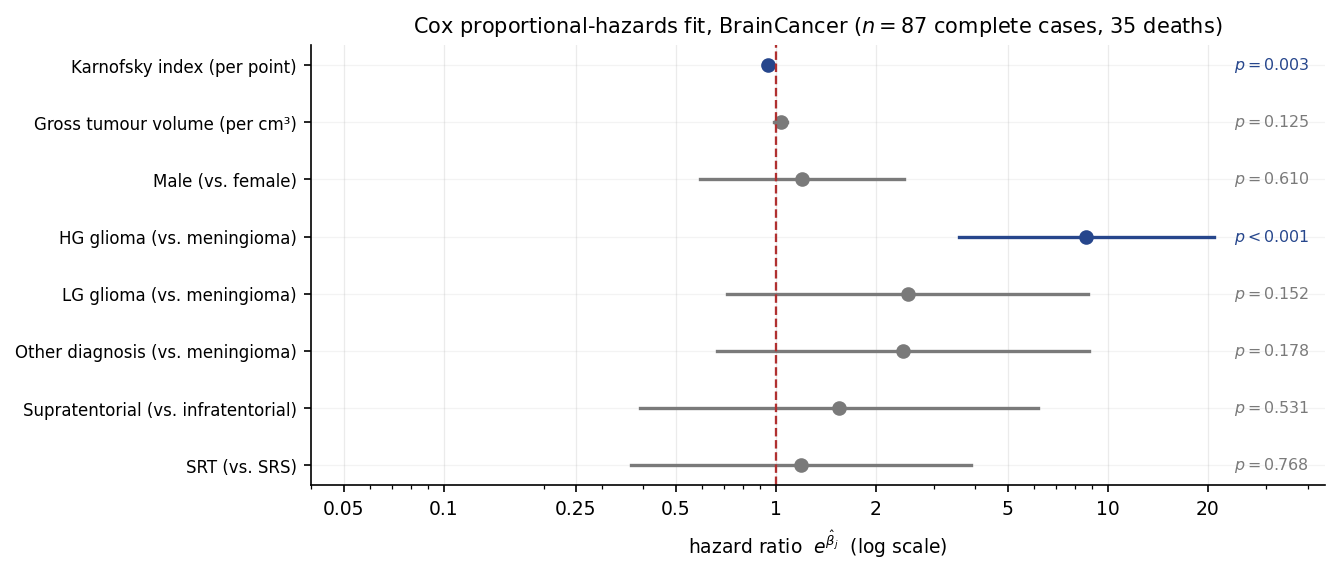
\includegraphics[width=0.94\textwidth,height=0.49\textheight,keepaspectratio]{ch11_forest.png}
  \end{center}
  \begin{takeaway}
    The vertical line at $\mathrm{HR}=1$ is ``no effect''; intervals are plotted on a
    \textbf{log} scale, which is the scale on which they are symmetric. Only two
    intervals clear the line: \texttt{ki} ($0.947$, just left of it) and HG glioma
    ($8.624$, far right). Six covariates, $35$ deaths --- most intervals are simply wide.
  \end{takeaway}
\end{frame}


\begin{frame}{Checking by eye}
  \footnotesize
  \begin{center}
    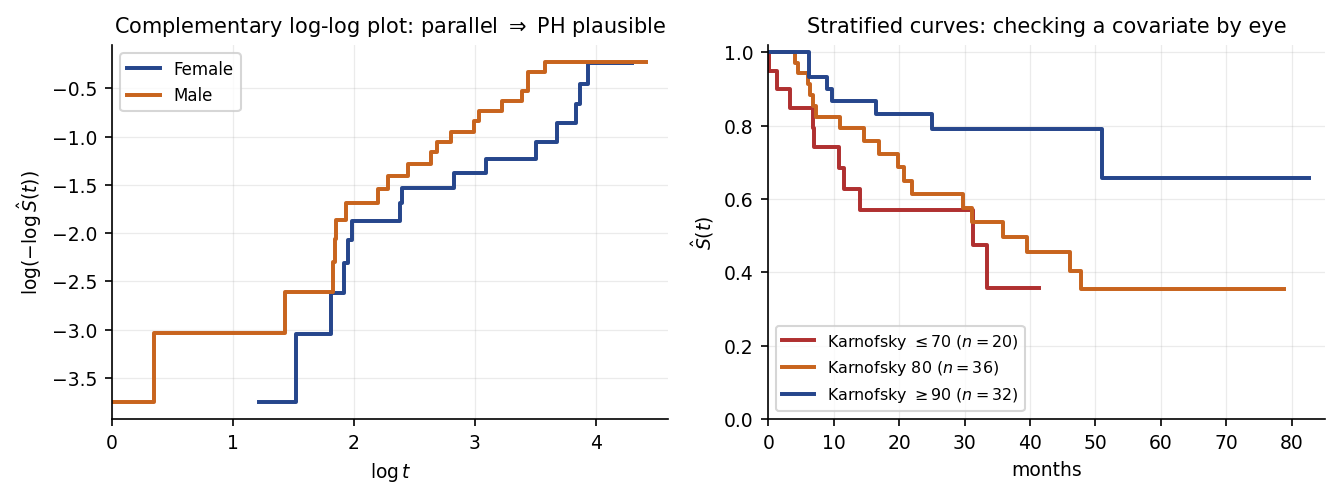
\includegraphics[width=0.94\textwidth,height=0.47\textheight,keepaspectratio]{ch11_loglog.png}
  \end{center}
  \begin{takeaway}
    Left: the two $\log(-\log\hat S)$ curves stay roughly parallel with a small constant
    gap, consistent with PH for \texttt{sex}. Right: stratifying by Karnofsky index gives
    three ordered, non-crossing curves ($n=20,36,32$) --- also what PH predicts. Neither
    plot proves the assumption; both would have shown a gross violation.
  \end{takeaway}
\end{frame}

\begin{frame}{Greenwood's formula}
  \scriptsize
  \begin{block}{Variance of the Kaplan--Meier estimator}
    \[
      \widehat{\mathrm{Var}}\bigl(\hat S(t)\bigr)
        \approx \hat S(t)^2 \sum_{k:\,t_k\le t}\frac{d_k}{r_k\,(r_k-d_k)} .
    \]
  \end{block}
  \begin{readme}[Sketch and how to use it]
    \begin{itemize}
      \item Write $\log\hat S(t)=\sum_k \log(1-d_k/r_k)$. Treat the $d_k$ as independent
            binomials given $r_k$, so $\widehat{\mathrm{Var}}(d_k/r_k)=
            \frac{(d_k/r_k)(1-d_k/r_k)}{r_k}$, propagate through the logarithm, and sum.
      \item Multiplying back by $\hat S(t)^2$ (the delta method) gives the formula.
      \item Each term grows as $r_k$ shrinks: that is precisely why the band widens to
            the right.
      \item Software reports a \emph{log--log-transformed} interval, so the endpoints stay
            inside $[0,1]$ and the interval is asymmetric.
    \end{itemize}
  \end{readme}
  \begin{numexample}[BrainCancer at 20 months]
    $\hat S(20)=0.7132$ and $\sum d_k/(r_k(r_k-d_k))=0.005101$, so
    $\mathrm{se}=0.7132\sqrt{0.005101}=0.0509$. The naive interval
    $0.7132\pm1.96(0.0509)=[0.613,0.813]$; \texttt{lifelines}' log--log interval is
    $[0.600,0.800]$ --- same information, better behaved near the boundaries.
  \end{numexample}
\end{frame}

\begin{frame}{Other censoring, and truncation}
  \footnotesize
  \begin{readme}[Four situations that are not right-censoring]
    \begin{itemize}
      \item \textbf{Left-censoring:} the event had already happened before observation
            began --- we know $T<Y$. Common in infection studies where a subject is
            already seropositive at enrolment.
      \item \textbf{Interval-censoring:} the event happened between two visits, so
            $T\in(a,b]$. Any periodically screened cohort produces this; treating the
            visit date as the event date biases times upwards.
      \item \textbf{Left-truncation (delayed entry):} a subject only enters the study
            after surviving to age $a$, so must be excluded from the risk set before $a$.
            Ignoring it makes survival look better than it is.
      \item \textbf{Competing risks:} death from another cause makes the event of interest
            unobservable forever. Kaplan--Meier on the cause of interest then
            \emph{overstates} incidence; use a cumulative-incidence function instead.
    \end{itemize}
  \end{readme}
  \begin{takeaway}
    Right-censoring is the easy case, and the one the chapter treats. The others
    need different likelihoods --- but the same discipline of asking exactly what
    each record proves.
  \end{takeaway}
\end{frame}

\begin{frame}{Deriving the partial likelihood, and ties}
  \footnotesize
  \begin{readme}[The risk-set argument]
    Condition on the fact that \emph{some} subject in $R(t_k)$ died at $t_k$, and ask which
    one. Under the Cox model the instantaneous rate for subject $j$ is
    $h_0(t_k)e^{x_j^\top\beta}$, so
    \[
      \Pr\bigl(\text{subject }i\text{ is the one}\bigr)
      =\frac{h_0(t_k)e^{x_i^\top\beta}}{\sum_{j\in R(t_k)}h_0(t_k)e^{x_j^\top\beta}}
      =\frac{e^{x_i^\top\beta}}{\sum_{j\in R(t_k)}e^{x_j^\top\beta}} .
    \]
    The nuisance $h_0(t_k)$ cancels because it is common to every subject at risk at that
    instant. Multiplying these conditional probabilities over all observed events gives
    $\mathrm{PL}(\beta)$; it is not a likelihood for the data, but it behaves like one.
  \end{readme}
  \begin{readme}[Ties]
    With continuous time, ties have probability zero; with monthly or daily data they are
    everywhere. \textbf{Breslow}: use the same denominator for all tied events (fast,
    biased towards $0$ when ties are heavy). \textbf{Efron}: discount the denominator
    progressively across the tied set (the \texttt{lifelines} default, and nearly always
    the better choice). \textbf{Exact}: average over all orderings --- correct and
    expensive.
  \end{readme}
\end{frame}

\begin{frame}{The log-rank test is a score test of the Cox model}
  \scriptsize
  \begin{readme}[Why the chapter's two headline methods are one]
    Fit a Cox model with a single binary covariate $x_i=\mathbf{1}\{i\in\text{group }1\}$.
    The score of the partial log-likelihood at $\beta=0$ is
    \[
      \left.\frac{\partial \log\mathrm{PL}}{\partial\beta}\right|_{\beta=0}
      = \sum_k\Bigl(d_{1k}-d_k\frac{r_{1k}}{r_k}\Bigr) = O_1-E_1 ,
    \]
    and the corresponding information is $V_1$ (with Breslow's tie handling). So the score
    test $(O_1-E_1)^2/V_1$ \textbf{is} the log-rank statistic.
  \end{readme}
  \begin{numexample}[BrainCancer split by sex]
    Log-rank: $\chi^2_1=1.4405$, $p=0.2301$. Cox with \texttt{sex} alone:
    $\hat\beta=0.4077$ ($\mathrm{HR}=1.503$), Wald $z=1.192$ giving $p=0.2333$, and a
    likelihood-ratio test of $1.4388$, $p=0.2303$. Three asymptotically equivalent tests
    of the same null, agreeing to two decimals.
  \end{numexample}
  \begin{takeaway}
    The log-rank test is the assumption-light special case; Cox is the general
    machine. That is also why the log-rank test inherits Cox's blind spot for
    crossing hazards.
  \end{takeaway}
\end{frame}

\begin{frame}{Time-varying covariates and immortal-time bias}
  \footnotesize
  \begin{readme}[The setup]
    Some covariates change during follow-up: a patient starts a drug at month $7$, a
    customer upgrades at month $14$. The Cox model handles this by letting $x_i(t)$ enter
    the risk set as it is \emph{at that instant}:
    $h(t\mid x_i(t))=h_0(t)\exp\{x_i(t)^\top\beta\}$, fitted from a data set split into
    one row per subject per interval.
  \end{readme}
  \begin{mistake}[Immortal-time bias]
  \scriptsize
    Classifying a subject as ``treated'' from time zero when treatment only began at month
    $7$ grants them seven months during which they \emph{could not} have been classified as
    an untreated death. Treatment then looks protective purely by construction --- an
    error that has produced real and repeatedly retracted findings on statins, screening
    and adherence.
  \end{mistake}
  \begin{takeaway}
    A covariate may only use information available at the time it is applied. If the
    exposure has a start date, the analysis must have one too.
  \end{takeaway}
\end{frame}

\begin{frame}{Exercise 11.7 --- The exponential model [Math]}
\begin{exercise}
  Suppose $T$ has a constant hazard, $h(t)=\lambda$ for all $t>0$.
  \begin{enumerate}
    \item Derive $H(t)$ and $S(t)$.
    \item Find the median survival time in terms of $\lambda$.
    \item Show that this family satisfies proportional hazards when
          $\lambda_i=\lambda_0e^{x_i^\top\beta}$, and identify the baseline hazard.
    \item With $n$ subjects, $D=\sum_i\delta_i$ events and total follow-up
          $\sum_i Y_i$, the maximum-likelihood estimator is
          $\hat\lambda=D/\sum_i Y_i$. Evaluate it for BrainCancer ($D=35$,
          $\sum_i Y_i=2416.26$ months) and compare the implied median with the
          Kaplan--Meier median of $47.8$.
  \end{enumerate}
\end{exercise}
\end{frame}

\begin{frame}{Solution --- Exercise 11.7}
\begin{solutionbox}
  \scriptsize
  \textbf{Part 1.} $H(t)=\int_0^t\lambda\,du=\lambda t$, so
  $S(t)=e^{-H(t)}=e^{-\lambda t}$: the exponential distribution, the unique
  memoryless survival law.

  \medskip
  \textbf{Part 2.} Solve $e^{-\lambda t}=0.5$: \
  $t_{0.5}=\dfrac{\log 2}{\lambda}=\dfrac{0.6931}{\lambda}$.

  \medskip
  \textbf{Part 3.} With $\lambda_i=\lambda_0e^{x_i^\top\beta}$ the hazard is
  $h(t\mid x_i)=\lambda_0e^{x_i^\top\beta}$, which is exactly
  $h_0(t)e^{x_i^\top\beta}$ with the \emph{constant} baseline $h_0(t)\equiv\lambda_0$.
  The ratio of two hazards is $e^{(x_i-x_j)^\top\beta}$, free of $t$: an exponential model
  is a Cox model with the baseline pinned down.

  \medskip
  \textbf{Part 4.} $\hat\lambda=35/2416.26=0.014485$ deaths per month of follow-up, so the
  implied median is $\log 2/0.014485=47.85$ months --- strikingly close to the
  Kaplan--Meier value of $47.8$. Reassuring, but partly luck: the constant-hazard
  assumption spans nearly seven years, and the two estimates diverge at other quantiles.
\end{solutionbox}
\begin{mistake}
  \scriptsize
  Estimating $\lambda$ as $D/n$ or as $1/\bar Y$ over events only. The denominator
  must be \textbf{total time at risk}, $\sum_i Y_i$, which is what censored subjects
  contribute.
\end{mistake}
\end{frame}

\end{document}
